%!TEX program = xelatex
\documentclass[11pt, a4paper]{article}

\usepackage{amsmath}
\usepackage{amssymb}

% fonts
\usepackage{xeCJK}
\setCJKmainfont[BoldFont=SimHei]{SimSun}
\setCJKfamilyfont{hei}{SimHei}
\setCJKfamilyfont{kai}{KaiTi}
\setCJKfamilyfont{fang}{FangSong}
\newcommand{\hei}{\CJKfamily{hei}}
\newcommand{\kai}{\CJKfamily{kai}}
\newcommand{\fang}{\CJKfamily{fang}}

% style
\usepackage[top=2.54cm, bottom=2.54cm, left=3.18cm, right=3.18cm]{geometry}
\linespread{1.5}
\usepackage{indentfirst}
\parindent 2em
\punctstyle{quanjiao}
\renewcommand{\today}{\number\year 年 \number\month 月 \number\day 日}

% figures and tables
\usepackage{graphicx}
\usepackage[font={bf, footnotesize}, textfont=md]{caption}
\makeatletter
    \newcommand\fcaption{\def\@captype{figure}\caption}
    \newcommand\tcaption{\def\@captype{table}\caption}
\makeatother
\usepackage{booktabs}
\renewcommand\figurename{图}
\renewcommand\tablename{表}
\newcommand{\fref}[1]{\textbf{图 \ref{#1}}}
\newcommand{\tref}[1]{\textbf{表 \ref{#1}}}
\newcommand{\tabincell}[2]{\begin{tabular}{@{}#1@{}}#2\end{tabular}} % multiply lines in one grid
\usepackage{longtable} % long table

\usepackage{listings}
\lstset{basicstyle=\ttfamily}

\usepackage{xcolor}
\renewcommand{\r}{\color{red}}
\usepackage{tabulary}
% start of document
\title{\textbf{MIPS-16E流水CPU实验报告}}
\author{
    \kai 钱迪晨 \quad 计35 \quad 2013011402 \\
    \kai 叶子鹏 \quad 计35 \quad 2013011404 \\
    \kai 朱俸民 \quad 计35 \quad 2012011894
}
\date{\kai\today}

% -----------------start here------------------%
\begin{document}

\maketitle

\section{概述}

我们实现了一个无延迟槽的带动态分支预测的流水线CPU。我们实现了一个通用性极佳(支持软硬件中断,支持绘图)的计算机。

我们最初的目的是尽可能不插,少插气泡,由于某些冲突必须暂停流水线,我们最终仅在3种情况插1个气泡,而绝大多数时候我们都无需插气泡。我们的CPU的主频最高可以达到21M(我们使用了ISE自带的模拟器件IP核DCM来分频)对于老师给的5个测例,我们花费的时间都非常少,因为我们几乎不用插气泡,所以花费的时间约等于指令数除以主频。

为了提高运行效率,我们增加了分支预测功能,branch指令和jump指令均在decode阶段进行,从而使得因为跳转引入的气泡尽可能的少。分支预测采取的是一个大小为3的查询表,每次使用pc进行查询,如果出现一次错误则更新,即记录上一次的结果。

除了CPU的核心以外,我们做了硬件中断,软件中断,像素映射的VGA接口的显示器(由于片内的RAM容量不大,不足以存下RGB,我们的显示是蓝白的)。

由于我们是像素映射,硬件的接口不仅单一而且不利于编程(非常繁琐,由于屏幕非常大,不足以用16位表示坐标,我们得传2次参数才能确定一个点),我们用软件实现了如下几个画图的接口:(详见第六节)

\begin{enumerate}
    \item 画一个点
    \item 画一条细线段
    \item 画一条粗线段
    \item 画一个等腰直角三角形
    \item 从数据RAM中读取一个形状(用于实现字符集,比如Unicode或者ASCII)
\end{enumerate}

\section{特色}


\begin{enumerate}
    \item \textbf{多条旁路}
    \item \textbf{动态分支预测}
    \item \textbf{消除延迟槽}:我们所有的跳转指令都不需要延迟槽,也不会暂停流水线
    \item \textbf{内存统一编址}
    \item \textbf{外设·键盘}:一个支持字母,数字,空格,退格,回车,shift组合键的键盘
    \item \textbf{支持硬件中断}:支持键盘触发硬件中断,为其他设备触发硬件中断留下了接口
    \item \textbf{支持软件中断}:支持软件中断scanf
    \item \textbf{外设·屏幕}:像素映射的屏幕,我们提供了字符和图形的库
    \item \textbf{支持绘图}:比字符映射的屏幕更通用
    \item \textbf{库支持}:我们用汇编写了总共千行的代码,提供了丰富的库
    \item \textbf{专用的Term}:我们为自己打造了专用的Term,方便调试,更方便展示
\end{enumerate}
\section{具体实现}

\subsection{CPU模块}

CPU模块无可厚非是我们本次实现中最重要的一个模块,这个模块里面包含了非常多的原件,我们使用了如下组件来实现我们整个CPU。下面会一一列举。

\begin{center}
    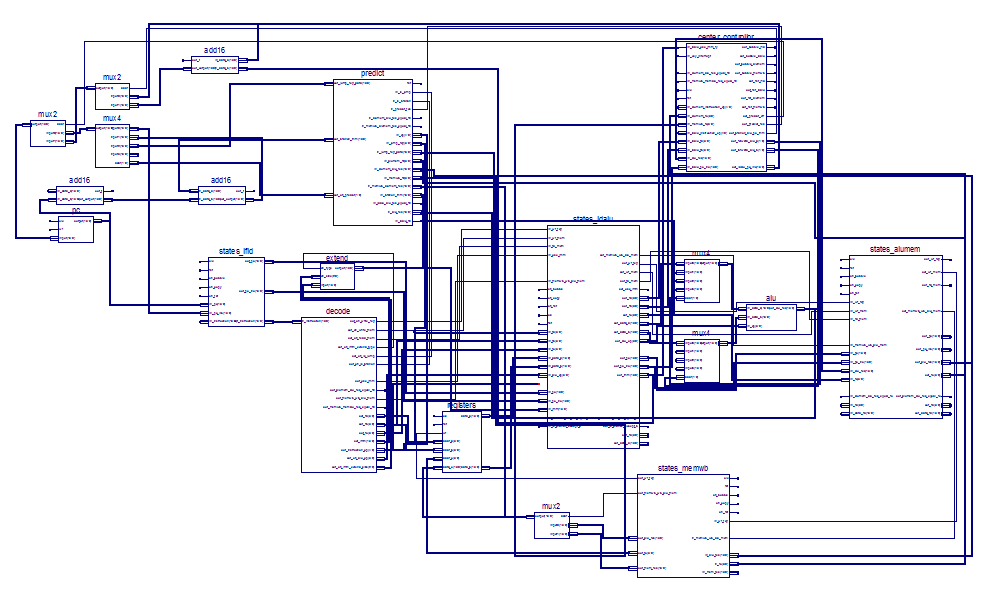
\includegraphics[width=14cm]{image/detail/detail_cpu.png}
    \fcaption{CPU结构图}\label{fig:cpu_structure}
\end{center}

\subsubsection{锁存单元}

锁存单元包含if/id阶段,id/alu阶段,alu/mem阶段,mem/wb阶段四个大的锁存器,在上升沿触发。这几个锁存器的行为都受到中央控制单元的控制,中央控制单元可以命令其进行气泡的插入,以及重置功能。

这四个部件的图如\fref{fig:ifid}-\fref{fig:idalu}所示,具体信号如\tref{table:ifid}-\tref{table:idalu}所示。

\begin{center}
    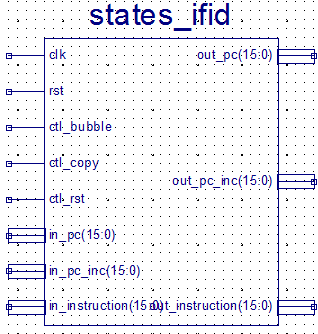
\includegraphics[width=7cm]{image/detail/detail_ifid.png}
    \fcaption{IF/ID阶段锁存器设计图}\label{fig:ifid}
\end{center}

\begin{center}
    \tcaption{IF/ID阶段锁存器信号}\label{table:ifid}
    \begin{longtable}{p{0.2\columnwidth}p{0.8\columnwidth}}
        \toprule
        信号 & 信号描述 \\
        \midrule
        clk & cpu的时钟信号,上升沿的时候根据ctl\_bubble和ctl\_rst进行控制。如果ctl\_bubble和ctl\_rst均为低电平则进行锁存,将in\_pc, in\_pc\_inc, in\_instruction进行锁存并输出。 \\
        rst & 异步清空信号,由外部控制开关接入。 \\
        ctl\_bubble & 气泡控制信号,由中央控制单元给出,如果该信号为高电平则表示下一个时钟上升沿,输出数据保持不变,低电平则该控制无效。 \\
        ctl\_copy &  由中央控制单元给出,用来进行数据拷贝。\\
        ctl\_rst & 重置控制信号,由中央控制单元给出,如果如果该信号为高电平则表示下一个时钟输出清空即为一条NOP指令,低电平则该控制无效。 \\
        in\_pc & 表示下一条将要锁存的指令的pc。 \\
        in\_pc\_inc & 表示下一条将要锁存的指令的pc+1。 \\
        in\_instruction & 表示下一条将要锁存的指令内容 \\
        out\_pc & 表示已经锁存的指令的pc。 \\
        out\_pc\_inc & 表示已经锁存的指令的pc+1。 \\
        out\_instruction & 表示已经锁存的指令。 \\
        \bottomrule
    \end{longtable}
\end{center}

\begin{center}
    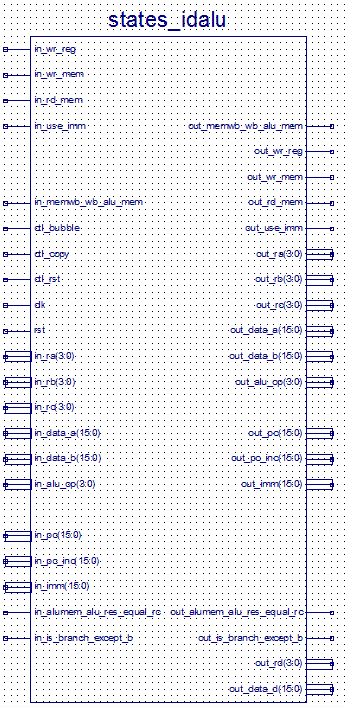
\includegraphics[width=8cm]{image/detail/detail_idalu.png}
    \fcaption{ID/ALU阶段锁存器设计图}\label{fig:idalu}
\end{center}

\begin{center}
    \tcaption{ID/ALU阶段锁存器信号}\label{table:idalu}
    \begin{longtable}{p{0.2\columnwidth}p{0.8\columnwidth}}
        \toprule
        信号 & 信号描述 \\
        \midrule
        in\_ra  & 这是下一条指令decode出来的alu操作数a的寄存器值,注意不是数值,会传递给中央控制单元进行旁路选择。 \\
        % 用来传输给选择器最后送到alu进行计算
        in\_rb &  这是下一条指令decode出来的alu操作数b的寄存器值,注意不是数值,会传递给中央控制单元进行旁路选择。\\
        in\_rc &  这是下一条指令decode出来的寄存器c的值,注意不是数值,会传递给中央控制单元进行旁路选择,也会传递给alumem锁存器。c的寄存器表示的
        是写回的寄存器,非常重要,所以要一直往后传。\\
        in\_data\_a &  这是下一条指令decode出来的alu操作数a的值,用来传输给选择器,(选择器可能会选择旁路),最后送到alu进行计算。 \\
        in\_data\_b &  这是下一条指令decode出来的alu操作数b的值,用来传输给选择器,(选择器可能会选择旁路),最后送到alu进行计算。 \\\\
        in\_alu\_op &  这是下一条指令alu的操作码,会传输给三个alu,具体内容请看alu部分。\\
        in\_pc &  表示下一条将要锁存的指令的pc。\\
        in\_pc\_inc &  表示下一条将要锁存的指令的pc+1。\\
        in\_imm &  表示下一条将要锁存的decode出来的立即数。\\
        in\_wr\_reg &  表示下一条指令是否需要在writeback阶段写回寄存器。\\
        in\_wr\_mem &  表示下一条指令是否需要在memory阶段写内存。\\
        in\_rd\_mem &  表示下一条指令是否需要在memory阶段读内存。\\
        in\_use\_imm & 表示下一条指令在alu阶段是否需要使用立即数,这个信号会帮助中央控制单元进行alu\_data\_b旁路的控制。 \\
        in\_alumem\_alu\_  res\_equal\_rc &  表示下一条指令到memory阶段的时候,alu的出的结果是否会在writeback阶段写回寄存器。这个信号也是为了帮助中央控制单元进行旁路控制。\\
        in\_memwb\_wb\_  alu\_mem &  表示下一条指令在writeback阶段写回的数据是memory阶段读出的数据,还是在alu阶段算出的结果。\\
        in\_is\_branch\_  except\_b & 表示下一条指令是否是branch指令,除了b指令以外的branch指令都是高电平,这个信号是帮助中央控制单元进行分支预测的检验使用的信号。 \\
        ctl\_bubble &  气泡控制信号,由中央控制单元给出,如果该信号为高电平则表示下一个时钟上升沿,输出数据保持不变,低电平则该控制无效。\\
        ctl\_copy &  由中央控制单元给出,用来进行数据拷贝。\\
        ctl\_rst &  重置控制信号,由中央控制单元给出,如果如果该信号为高电平则表示下一个时钟输出清空即为一条NOP指令,低电平则该控制无效。\\
        clk &  cpu的时钟信号,上升沿的时候根据ctl\_bubble和ctl\_rst进行控制。如果ctl\_bubble和ctl\_rst均为低电平则进行锁存,将所有带有out前轴的信号对应的in信号锁存然后输出。\\
        rst &  异步清空信号,由外部控制开关接入。\\
        out\_ra &  表示alu阶段运算的寄存器a的值,这个值会送到中央控制单元进行旁路的控制。\\
        out\_rb &  表示alu阶段运算的寄存器b的值,这个值会送到中央控制单元进行旁路的控制。\\
        out\_rc &  表示writeback阶段写回的寄存器c的值。\\
        out\_rd &  rd是一个特殊的输出,只会在sw这条指令进行使用,rd也需要送到中央控制单元进行旁路的控制,他的内容和rb完全一致。\\
        out\_data\_a &  表示alu阶段运算a的值,这个值是从一个四选一的选择器得到的,这个选择器的控制由中央控制单元给出。\\
        out\_data\_b &  表示alu阶段运算b的值,这个值是从一个四选一的选择器得到的,这个选择器的控制由中央控制单元给出。\\
        out\_data\_d &  表示memory阶段sw指令可能用到的值,这个值是从一个四选一的选择器得到的,这个选择器的控制由中央控制单元给出。\\
        out\_alu\_op &  表示当前alu进行的运算符号。\\
        out\_pc &  表示已经锁存的指令的pc。\\
        out\_pc\_inc &  表示已经锁存的指令的pc+1。\\
        out\_imm &  表示已经锁存的指令的立即数,这个数字会连接到alu\_data\_b的选择器。\\
        out\_alumem\_alu\_  res\_equal\_rc &  表示当前指令到memory阶段的时候,alu的出的结果是否会在writeback阶段写回寄存器。这个信号也是为了帮助中央控制单元进行旁路控制。\\
        out\_memwb\_wb\_  alu\_mem &  表示当前指令在writeback阶段写回的数据是memory阶段读出的数据,还是在alu阶段算出的结果。\\
        out\_is\_branch\_  except\_b &  表示当前指令是否是branch指令,除了b指令以外的branch指令都是高电平,这个信号是帮助中央控制单元进行分支预测的检验使用的信号。\\
        out\_wr\_reg &  表示当前指令是否需要在writeback阶段写回寄存器。\\
        out\_wr\_mem &  表示当前指令是否需要在memory阶段写内存。\\
        out\_rd\_mem &  表示当前指令是否需要在memory阶段读内存。\\
        out\_use\_imm & 表示当前指令在alu阶段是否需要使用立即数,这个信号会帮助中央控制单元进行alu\_data\_b旁路的控制。 \\
        \bottomrule
    \end{longtable}
\end{center}

\begin{center}
    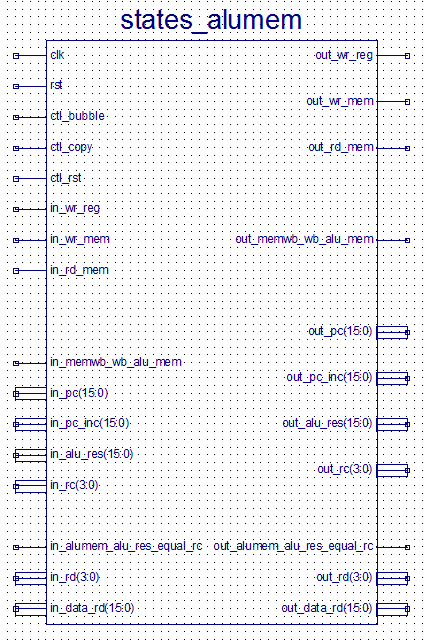
\includegraphics[width=8cm]{image/detail/detail_alumem.png}
    \fcaption{ALU/MEM阶段锁存器设计图}\label{fig:alumem}
\end{center}

\begin{center}
    \tcaption{ALU/MEM阶段锁存器信号}\label{table:alumem}
    \begin{longtable}{p{0.2\columnwidth}p{0.8\columnwidth}}
        \toprule
        信号 & 信号描述 \\
        \midrule
        in\_rc &  这是下一条指令decode出来的寄存器c的值,注意不是数值,会传递给中央控制单元进行旁路选择,也会传递给memwb锁存器。c的寄存器表示的
        是写回的寄存器,非常重要,所以要一直往后传。\\
        in\_rd & 这是专门为了sw指令设计的寄存器的值。\\
        in\_data\_rd & 这是专门为了sw指令设计的寄存器的值,通过一个4️选1选择可以确保数据的正确性。由于我们的设计问题,alu在进行sw指令的时候无法将sw的源寄存器值进行旁路计算解决数据冲突,所以使用了单独的一条旁路来解决这个问题。\\
        in\_pc &  表示下一条将要锁存的指令的pc。\\
        in\_pc\_inc &  表示下一条将要锁存的指令的pc+1。\\
        in\_wr\_reg &  表示下一条指令是否需要在writeback阶段写回寄存器。\\
        in\_wr\_mem &  表示下一条指令是否需要在memory阶段写内存。\\
        in\_rd\_mem &  表示下一条指令是否需要在memory阶段读内存。\\
        in\_alu\_res & 表示下一条指令alu得出的结果。\\


        in\_alumem\_alu\_  res\_equal\_rc & 表示下一条指令alu计算出的结果是否会在writeback阶段写回寄存器。这个信号也是为了帮助中央控制单元进行旁路控制。\\
        in\_memwb\_wb\_  alu\_mem & 表示下一条指令在writeback阶段写回的数据是memory阶段读出的数据,还是在alu阶段算出的结果。\\
        clk & cpu的时钟信号,上升沿的时候根据ctl\_bubble和ctl\_rst进行控制。如果ctl\_bubble和ctl\_rst均为低电平则进行锁存,将所有带有out前轴的信号对应的in信号锁存然后输出。\\
        rst & 异步清空信号,由外部控制开关接入。\\
        ctl\_bubble &  气泡控制信号,由中央控制单元给出,如果该信号为高电平则表示下一个时钟上升沿,输出数据保持不变,低电平则该控制无效。\\
        ctl\_copy &  由中央控制单元给出,用来进行数据拷贝。\\
        ctl\_rst &  重置控制信号,由中央控制单元给出,如果如果该信号为高电平则表示下一个时钟输出清空即为一条NOP指令,低电平则该控制无效。\\
        out\_pc &  表示已经锁存的指令的pc。\\
        out\_pc\_inc &  表示已经锁存的指令的pc+1。\\
        out\_alu\_res & 表示当前指令在alu阶段通过alu计算出来的值。\\
        out\_rc & 表示当前指令decode出来的目的寄存器c的值。\\
        out\_wr\_reg &  表示当前指令是否需要在writeback阶段写回寄存器。\\
        out\_wr\_mem &  表示当前指令是否需要在memory阶段写内存。\\
        out\_rd\_mem &  表示当前指令是否需要在memory阶段读内存。\\
        out\_memwb\_wb\_  alu\_mem & 表示当前指令在writeback阶段写回的数据是memory阶段读出的数据,还是在alu阶段算出的结果。\\
        \bottomrule
    \end{longtable}
\end{center}

\begin{center}
    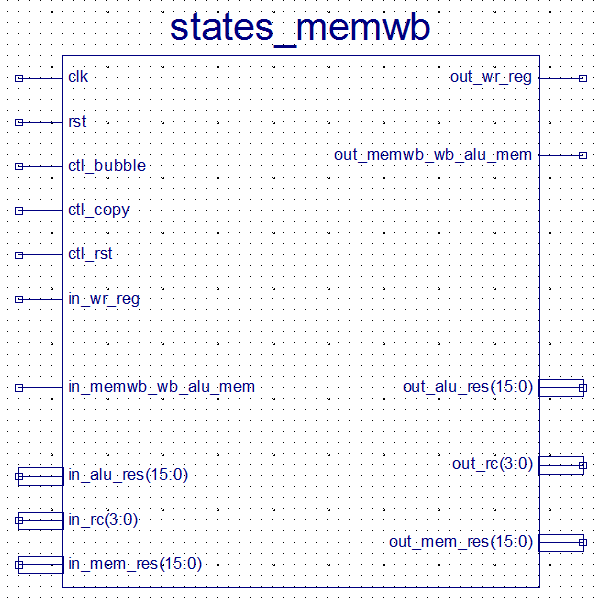
\includegraphics[width=8cm]{image/detail/detail_memwb.png}
    \fcaption{MEM/WB阶段锁存器设计图}\label{fig:memwb}
\end{center}

\begin{center}
    \tcaption{MEM/WB阶段锁存器信号}\label{table:memwb}
    \begin{longtable}{p{0.2\columnwidth}p{0.8\columnwidth}}
        \toprule
        信号 & 信号描述 \\
        \midrule
        clk & cpu的时钟信号,上升沿的时候根据ctl\_bubble和ctl\_rst进行控制。如果ctl\_bubble和ctl\_rst均为低电平则进行锁存,将所有带有out前轴的信号对应的in信号锁存然后输出。\\
        rst & 异步清空信号,由外部控制开关接入。\\
        ctl\_bubble &  气泡控制信号,由中央控制单元给出,如果该信号为高电平则表示下一个时钟上升沿,输出数据保持不变,低电平则该控制无效。\\
        ctl\_copy &  由中央控制单元给出,用来进行数据拷贝。\\
        ctl\_rst &  重置控制信号,由中央控制单元给出,如果如果该信号为高电平则表示下一个时钟输出清空即为一条NOP指令,低电平则该控制无效。\\
        in\_alu\_res & 表示下一条指令alu阶段计算出来的结果,可能用于写回。\\
        in\_rc & 表示下一条指令写回的寄存器值。\\
        in\_wr\_reg & 表示下一条指令是否写回寄存器。\\
        in\_mem\_res & 表示下一条指令memory阶段得到的结果。\\
        in\_memwb\_wb\_ alu\_mem & 表示下一条指令写回寄存器堆的是alu计算的结果还是memory访存的结果。\\
        out\_wr\_reg & 当前指令用来控制寄存器堆的写使能信号,使其可以在下降沿的时候更新。\\
        out\_memwb\_wb\_ alu\_mem & 当前指令写回内容2选1的控制信号,是选择alu计算的结果还是memory访存的结果。\\
        \bottomrule
    \end{longtable}
\end{center}

\subsubsection{PC锁存单元}
    PC锁存器,用来锁存PC,保证PC的改写受到中央控制部分的控制。我们规定在下降沿写入,组合逻辑输出。
    具体信号请看下表。

\begin{center}
    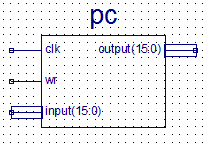
\includegraphics[width=6cm]{image/detail/detail_pc.png}
    \fcaption{PC锁存器}\label{fig:pc}
\end{center}
\begin{center}
    \tcaption{PC锁存器}\label{table:pc}
    \begin{longtable}{p{0.2\columnwidth}p{0.8\columnwidth}}
        \toprule
        信号 & 信号描述 \\
        \midrule
            input & 表示修改信号的输入,即修改的值。\\
            clk & CPU时钟。\\
            wr & 修改使能,如果为高电平则在下降沿修改pc的锁存器的值。\\
            rst & 异步清空信号,由外部控制开关接入。\\
            output & 当前pc锁存的值,组合逻辑。\\
        \bottomrule
    \end{longtable}
\end{center}

下一条PC的选择是一个非常复杂的结构,具体的原理图如下。
\begin{center}
    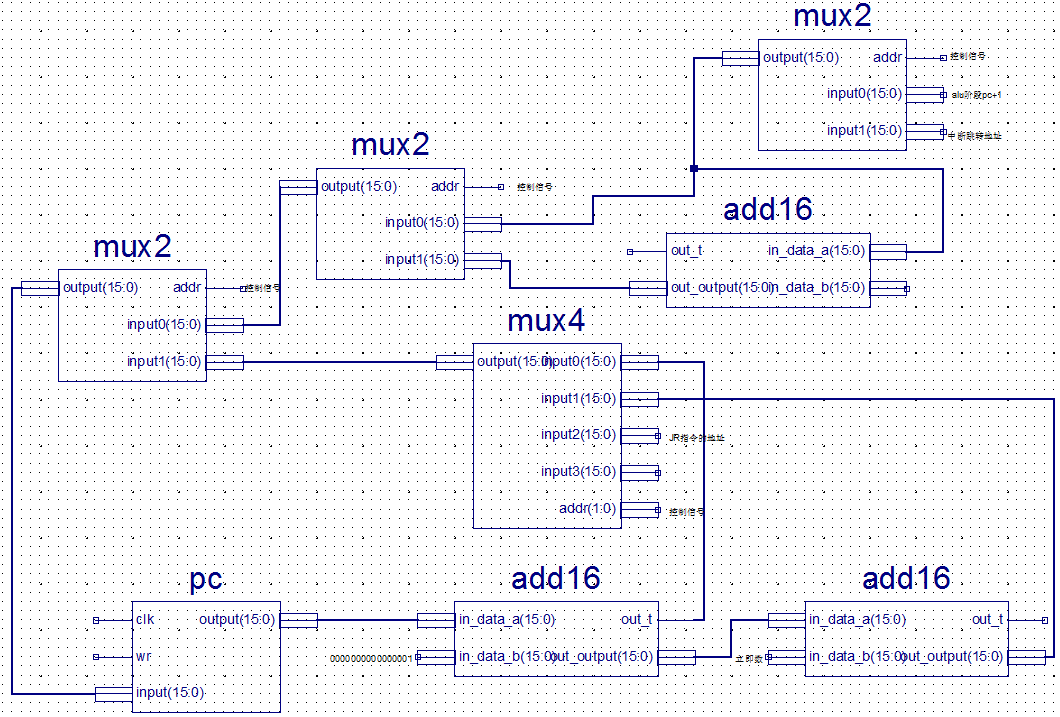
\includegraphics[width=14cm]{image/detail/detail_pc_structure.png}
    \fcaption{PC结构图}\label{fig:pcstructure}
\end{center}
具体而言,PC的选择由两条路线决定。
\begin{enumerate}
    \item 在decode阶段进行的跳转,包含jr指令以及分支预测。这里使用了图中下部分的部件,4选1的选择器可以选择pc+1,pc+1+imm,reg的值进行跳转。控制信号都是中央控制单元给出的。
    \item 在alu发现分支预测错误或者进行中断的跳转,则在上部分,最右边是一个2选1,选择进行跳转的基础地址是alu阶段的记录下来的pc地址,或者是中断的指令的地址,左边的2选1则是是否加上立即数的选择器,最后连向最左边的2选1选择器。
\end{enumerate}
综合上面的结构,构成了我们的pc整个模块,是的cpu的跳转可以正常的工作。
由于大部分控制信号都是有中央控制单元给出,控制信号将统一在中央控制器里面描述。

\subsubsection{跳转单元}
    跳转单元,用来在decode阶段进行计算和控制跳转的目的地址,这里面有旁路来处理JR指令的数据冲突。
    具体信号请看下表。
\begin{center}
    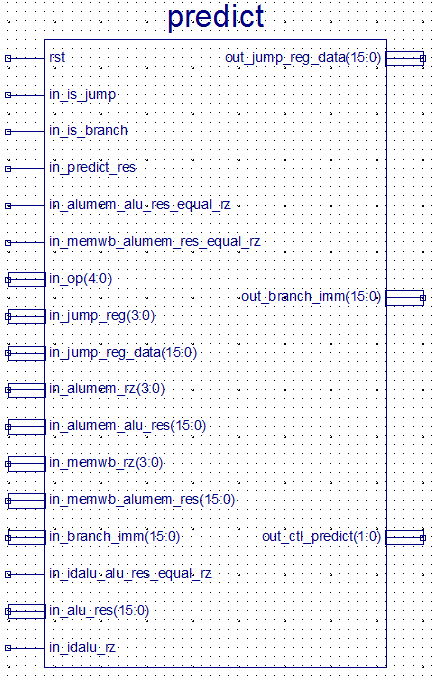
\includegraphics[width=8cm]{image/detail/detail_predict.png}
    \fcaption{跳转单元}\label{fig:predict}
\end{center}
\begin{center}
    \tcaption{跳转单元}\label{table:predict}
    \begin{longtable}{p{0.2\columnwidth}p{0.8\columnwidth}}
        \toprule
        信号 & 信号描述 \\
        \midrule
            rst & 异步清空信号,由外部控制开关接入。\\
            in\_is\_jump & 由decode给出的当前指令是不是jump指令。\\
            in\_is\_b & 由decode给出的当前指令是不是b指令。\\
            in\_is\_branch\_  except\_b & 由decode给出的当前指令是不是除了b的branch指令。 \\
            in\_predict\_res & 由中央控制单元给出的分支预测的结果。\\
            in\_jump\_reg & 由decode给出的jr指令的寄存器的值。\\
            in\_jump\_reg\_  data & 由寄存器堆给出的jr指令的寄存器的数据。\\
            in\_idalu\_alu\_  res\_equal\_rc & 这是为旁路设计的,用来计算alu阶段出现的数据冲突,这个信号表示alu阶段alu的值会在最后写回c寄存器。\\
            in\_idalu\_rc & 当前alu阶段c寄存器的值。\\
            in\_alu\_res & 当前alu阶段alu的值。\\
            in\_alumem\_rc & 当前alu阶段c寄存器的值。\\
            in\_alumem\_alu\_  res\_equal\_rc & 这是为旁路设计的,用来计算mem阶段出现的数据冲突,这个信号表示mem阶段alu的值会在最后写回c寄存器。\\
            in\_alumem\_alu\_  res & 当前memory阶段alu的值。\\
            in\_memwb\_rc & 当前writeback写回的寄存器c的值。\\
            in\_memwb\_alume  m\_res\_equal\_rc & 这是为旁路设计的,用来计算mem阶段出现的数据冲突,这个信号表示writeback阶段alu或者mem的值会在最后写回c寄存器。\\
            in\_memwb\_alume  m\_res & writeback阶段写回的值。\\
            in\_branch\_imm & 这个数据表示branch指令立即数的值,将会给pc模块用来进行加法。\\
            out\_jump\_reg\_  data & 这个输出用来连接到pc模块里面的4选1选择器,表示jr指令的目的地值。\\
            out\_branch\_imm & 这个数据用来输出表示branch指令立即数的值,将会给pc模块用来进行加法。\\
            out\_ctl\_predict & 这个数据用来输出表示分支预测的结果,连接到选择器上。\\
        \bottomrule
    \end{longtable}
\end{center}


\subsubsection{寄存器堆}
    寄存器堆用来输出寄存器的值,以及在时钟下降沿提供修改寄存器值的功能。
    具体信号请看下表。
\begin{center}
    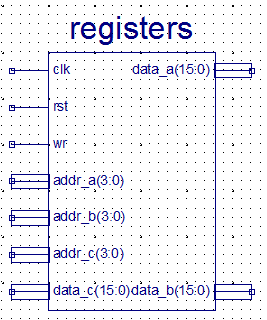
\includegraphics[width=6cm]{image/detail/detail_register.png}
    \fcaption{寄存器堆}\label{fig:register}
\end{center}
\begin{center}
    \tcaption{寄存器堆}\label{table:register}
    \begin{longtable}{p{0.2\columnwidth}p{0.8\columnwidth}}
        \toprule
        信号 & 信号描述 \\
        \midrule
            clk & CPU时钟信号。\\
            rst &  异步清空信号,由外部控制开关接入。\\
            wr & 寄存器堆写使能,如果为高电平则在clk下降沿的时候将data\_c写入对应的addr\_c里面。\\
            addr\_a & 接受decode出来的寄存器a。\\
            addr\_b & 接受decode出来的寄存器b。\\
            addr\_c & 接受writeback将要写回的寄存器c。\\
            data\_a & 输出decode出来的寄存器a的数值。\\
            data\_b & 输出decode出来的寄存器b的数值。\\
            data\_c & 写回阶段修改寄存器的值。\\
        \bottomrule
    \end{longtable}
\end{center}


\subsubsection{ALU}
    我们的ALU有一点不同,我们使用了三个ALU。
    Alu,Alu\_adds,Alu\_equal,分别是三个ALU。我们将ALU区分成三个的主要原因是为了减小延时。具体原因是因为Branch指令在ALU阶段受到数据冲突旁路的影响,可能导致延时非常大。而这里的瓶颈是中央控制单元的控制信号。
    中央控制单元修改Alu的数据选择的信号的延迟会非常大,而这个操作主要过程如下。
    \begin{enumerate}
        \item 中央控制单元由于受到memory和writeback阶段锁存的信号,修改Alu的data\_b的控制信号,也就是旁路的控制。
        \item Alu进行计算,结果返回中央控制单元。
        \item 中央控制单元检查是否和分支预测出现错误如果出现错误修改控制信号。
    \end{enumerate}
    具体内容请看下表。

\begin{center}
    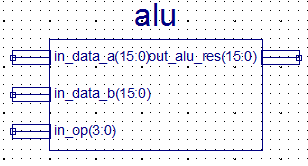
\includegraphics[width=6cm]{image/detail/detail_alu.png}
    \fcaption{算术逻辑单元}\label{fig:alu}
\end{center}
\begin{center}
    \tcaption{算术逻辑单元}\label{table:alu}
    \begin{longtable}{p{0.2\columnwidth}p{0.8\columnwidth}}
        \toprule
        信号 & 信号描述 \\
        \midrule
            in\_data\_a & alu的两个操作数之一。\\
            in\_data\_b & alu的两个操作数之一。\\
            in\_op & alu的操作码。\\
            out\_alu\_res & alu计算的结果。\\
        \bottomrule
    \end{longtable}
\end{center}


    为了处理数据冲突,in\_data\_a的输入是一个4选1的选择器,它有三种可能,控制信号由中央控制单元给出。
    \begin{enumerate}
        \item 寄存器堆给出的值,也就是alu阶段锁存器里面的值。
        \item memory阶段的alu计算结果,如果写回的寄存器和data\_a的寄存器一致的话。
        \item writeback阶段的alu或者memory得到的结果,如果写回的寄存器和data\_a的寄存器一致的话。
    \end{enumerate}


    同样,in\_data\_b的输入是一个4选1的选择器,它有四种可能,控制信号由中央控制单元给出。
    \begin{enumerate}
        \item 寄存器堆给出的值,也就是alu阶段锁存器里面的值。
        \item memory阶段的alu计算结果,如果写回的寄存器和data\_a的寄存器一致的话。
        \item writeback阶段的alu或者memory得到的结果,如果写回的寄存器和data\_a的寄存器一致的话。
        \item decode出来的立即数。
    \end{enumerate}

    ALU支持如下几种运算。
    \begin{enumerate}
        \item Alu\_adds支持加法,操作码为0000,为unsigned(A+B)。
        \item Alu支持减法,操作码为0001,为unsigned(A-B)。
        \item Alu支持逻辑左移,操作码为0011,为A<<B。
        \item Alu支持算术右移,操作码为0100,为A>>B。
        \item Alu支持异或,操作码为0101,为A  xor  B。
        \item Alu支持比较,操作码为0110,为A  ==  B。
        \item Alu支持符号比较,操作码为0111,为A  <=  B。
        \item Alu支持无符号比较,操作码为0111,为unsigned(A)  <=  unsigned(B)。
        \item Alu支持直接输出A,操作码为1000。
        \item Alu支持直接输出B,操作码为1001。
        \item Alu支持not,操作码为1010,为not  A。
        \item Alu\_equal支持和0比操作,操作码为1011,为A == 0。
        \item Alu\_equal支持和0比操作,操作码为1100,为A != 0。
        \item Alu支持not,操作码为1010,为not  A。
        \item Alu支持or,操作码为1011,为A  or  B。
        \item Alu支持and,操作码为1100,为A  and  B。
    \end{enumerate}

\subsubsection{译码器}
Decode用于翻译指令,生成一系列数据,并将数据传输给alu的锁存器或者跳转的控制器。
具体信号请看下表。

\begin{center}
    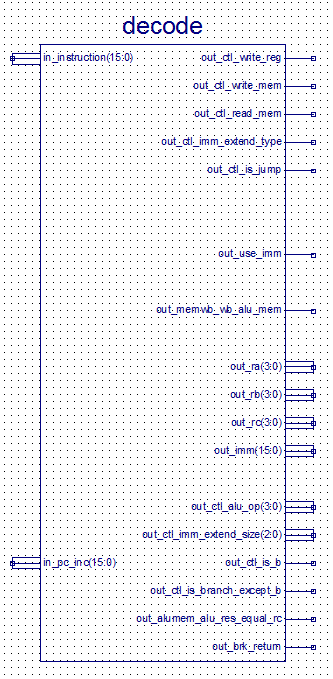
\includegraphics[width=8cm]{image/detail/detail_decode.png}
    \fcaption{译码器}\label{fig:decode}
\end{center}
\begin{center}
    \tcaption{译码器}\label{table:decode}
    \begin{longtable}{p{0.2\columnwidth}p{0.8\columnwidth}}
        \toprule
        信号 & 信号描述 \\
        \midrule
            in\_instruction & 输入的指令,用来进行decode。\\
            in\_pc\_inc & 当前指令的pc+1,mfpc这条指令就会使用pc+1当做立即数进行计算。\\
            out\_ra & 当前指令decode出来的寄存器a,用来进行alu计算。\\
            out\_rb & 当前指令decode出来的寄存器b,用来进行alu计算。\\
            out\_rc & 当前指令decode出来的寄存器c,当做目的寄存器,会在writeback里面进行写回。\\
            out\_ctl\_  write\_reg & 控制信号,如果是高电平则表示在writeback阶段需要对rc写回。\\
            out\_ctl\_  write\_mem & 控制信号,如果是高电平则表示在memory阶段需要写ram。\\
            out\_ctl\_  read\_mem & 控制信号,如果是高电平则表示在memory阶段需要读ram。\\
            out\_ctl\_alu\_op & alu阶段alu的操作码。\\
            out\_use\_imm & alu阶段,数据b是否使用立即数,这个信号是辅助中央控制单元进行控制的。\\
            out\_imm & 当前指令decode出来的立即数,需要经过extend模块进行扩展。\\
            out\_ctl\_imm  \_extend\_size & 控制信号,表示extend模块如何对立即数进行扩展,扩展立即数的大小。\\
            out\_ctl\_imm  \_extend\_type & 控制信号,表示extend模块如何对立即数进行扩展,扩展立即数是有符号还是无符号。\\
            out\_ctl\_is  \_jump & 控制指令,表示当前指令是不是j指令,传递到跳转模块。\\
            out\_ctl\_is  \_b & 控制指令,表示当前指令是不是b指令,传递到跳转模块。\\
            out\_ctl\_is  \_branch\_except\_b & 控制指令,表示当前指令是不是branch指令而不是b指令,传递到跳转模块和中央控制模块。\\
            out\_alumem\_  alu\_res\_equal\_rc & 控制信号,表示这条指令到memory阶段时候,alu的结果是不是会在writeback阶段写回寄存器c。这个信号是帮助中央控制单元进行旁路的控制的\\
            out\_memwb\_wb  \_alu\_mem & 控制信号,表示这条指令到writeback阶段时候,写回寄存器的数据是alu的结果还是访存的结果。\\
            out\_brk\_return & 这是中断返回的控制信号,传递给中央控制单元进行pc的跳转控制。\\
        \bottomrule
    \end{longtable}
\end{center}

\subsubsection{中央控制单元}
中央控制单元是最复杂的单元,里面包含了分支预测,中断的处理,以及所有控制信号的生成。这里先给出所有中央控制单元的信号。
\begin{center}
    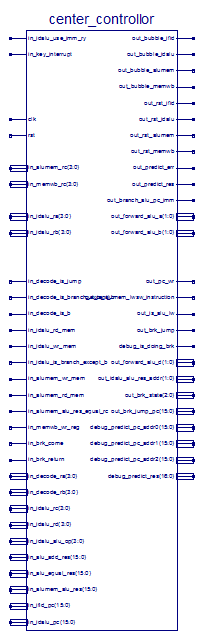
\includegraphics[width=7.3cm]{image/detail/detail_center_controllor.png}
    \fcaption{中央控制单元}\label{fig:center_controllor}
\end{center}
\begin{center}
    \tcaption{中央控制单元}\label{table:center_controllor}
    \begin{longtable}{p{0.2\columnwidth}p{0.8\columnwidth}}
        \toprule
        信号 & 信号描述 \\
        \midrule
            in\_decode\_ra & 这个是decode出来ra寄存器的值,这里如果发现decode出来的ra和已经在alu的指令有冲突,即alu的指令是lw,并且写回的寄存器是ra,那么这里会产生一系列控制,进行气泡的插入。\\
            in\_decode\_rb & 这个是decode出来rb寄存器的值,这里如果发现decode出来的rb和已经在alu的指令有冲突,即alu的指令是lw,并且写回的寄存器是ra,那么这里会产生一系列控制,进行气泡的插入。\\
            in\_decode\_is  \_jump & 这个信号表示decode出来的指令是不是jump指令,用处是,如果现在在memory阶段读写了instruction ram,则需要进行控制,控制的内容是保持ifid这个锁存器,并清除idalu的锁存器,具体原因是因为我们的设计导致读写instruction memory的时候pc给出的指令会出现错误,所以必须插气泡保证正确性。\\
            in\_decode\_is  \_branch\_except\_b & 这个信号表示decode出来的指令是不是branch指令,用处是,如果现在在memory阶段读写了instruction ram,则需要进行控制,控制的内容是保持ifid这个锁存器,并清除idalu的锁存器,具体原因是因为我们的设计导致读写instruction memory的时候pc给出的指令会出现错误,所以必须插气泡保证正确性。\\
            in\_decode\_is  \_b & 这个信号表示decode出来的指令是不是b指令,用处是,如果现在在memory阶段读写了instruction ram,则需要进行控制,控制的内容是保持ifid这个锁存器,并清除idalu的锁存器,具体原因是因为我们的设计导致读写instruction memory的时候pc给出的指令会出现错误,所以必须插气泡保证正确性。\\
            in\_idalu\_rd\_mem & 这个信号是alu阶段的指令是在memory读内存,用来帮助进行气泡控制的计算。\\
            in\_idalu\_wr\_mem & 这个信号是alu阶段的指令是在memory写内存,用来帮助进行气泡控制的计算。\\
            in\_idalu\_ra & 这个信号是alu阶段的指令的ra值,用来计算旁路的选择器。\\
            in\_idalu\_rb & 这个信号是alu阶段的指令的rb值,用来计算旁路的选择器。\\
            in\_idalu\_rc & 这个信号是alu阶段的指令的rc值,用来计算旁路的选择器。\\
            in\_idalu\_rd & 这个信号是alu阶段的指令的rd值,用来计算旁路的选择器。\\
            in\_idalu\_use\_ imm\_ry & 这个是alu阶段的指令,在decode的时候生成的信号,用来告诉中央控制单元是否要使用立即数,如果使用,那么alu\_data\_b就是立即数的值而不是寄存器堆里面读出来的值了。\\
            in\_idalu\_alu\_op & 这个是alu阶段的alu操作码,根据这个生成控制信号,控制三个alu的输出里面选择哪一个送到后续的模块里面。\\
            in\_alu\_add\_res & 这个是alu\_adds的结果,用来进行是否读写instruction memory的判断,如果是instruction memory的话需要进行气泡的插入。\\
            in\_alu\_equal\_res & 个是alu\_equal的结果,用来校验branch指令的结果是不是和分支预测的结果一致。\\
            in\_idalu\_is\_  branch\_except\_b & 这个是alu阶段指令是不是branch指令,告诉中央控制单元是否进行分支预测的校验。\\
            in\_alumem\_alu\_res & 这个是memory阶段alu的结果,用来帮助判断是否现在在读写instruction memory。\\
            in\_alumem\_rc & 这个是memory阶段的rc,用来帮助判断alu两个数据a和b的旁路的选择。\\
            in\_alumem\_wr  \_mem & 这个是memory阶段是否写内存的控制信号,用来帮助判断是否现在在读写instruction memory。\\
            in\_alumem\_rd  \_mem & 这个是memory阶段是否读内存的控制信号,用来帮助判断是否现在在读写instruction memory。\\
            in\_alumem\_alu\_  res\_equal\_rc & 这个是memory阶段的alu的结果是否会被写回寄存器的控制信号,用来帮助判断alu两个数据a和b的旁路的选择。\\
            in\_memwb\_rc & 这个是writeback阶段写回寄存器的值,用来帮助判断alu两个数据a和b的旁路的选择。\\
            in\_memwb\_wr\_reg & 这个是writeback阶段的alu或者memory的结果是否会被写回寄存器的控制信号,用来帮助判断alu两个数据a和b的旁路的选择。\\
            in\_brk\_come & 这个是中断的开始信号,具体中断的处理方法见后面。\\
            in\_ifid\_pc & 这个是ifid锁存器的pc,用来进行中断的跳回地址的计算。\\
            in\_idalu\_pc & 这个是idalu锁存器的pc,用来进行中断的跳回地址的计算。\\
            in\_brk\_return & 这个是中断结束的信号。用来帮助中央控制单元进行pc的调整,跳回。\\
            clk & CPU的时钟。\\
            rst & 异步清空信号,由外部控制开关接入。\\
            out\_bubble\_ifid & 这个是ifid锁存器的气泡控制信号。\\
            out\_bubble\_idalu & 这个是idalu锁存器的气泡控制信号。\\
            out\_bubble\_  alumem & 这个是alumem锁存器的气泡控制信号。\\
            out\_bubble\_  memwb & 这个是memwb锁存器的气泡控制信号。\\
            out\_rst\_ifid & 这个是ifid锁存器的重置控制信号。\\
            out\_rst\_idalu & 这个是idalu锁存器的重置控制信号。\\
            out\_rst\_alumem & 这个是alumem锁存器的重置控制信号。\\
            out\_rst\_memwb & 这个是memwb锁存器的重置控制信号。\\
            out\_forward\_  alu\_a & 这个是alu阶段数据a的4选1的控制信号。\\
            out\_forward\_  alu\_b & 这个是alu阶段数据b的4选1的控制信号。\\
            out\_forward\_  alu\_d & 这个是alu阶段数据d的4选1的控制信号。\\
            out\_predict\_err & 这个是pc模块里面最后一层2选1的控制信号,如果出现错误下一个pc则不由跳转模块决定,由中央控制模块决定,反之亦然。\\
            out\_predict\_res & 这个是输出给跳转单元的分支预测结果。\\
            out\_branch\_  alu\_pc\_imm & 这个是pc模块里面分支预测错误以后,alu阶段里面branch指令的立即数大小,用来进行新的pc的计算。\\
            out\_pc\_wr & 这个是pc的写使能。\\
        \bottomrule
    \end{longtable}
\end{center}

\subsubsection{旁路}
我们将旁路的选择设计在中央控制器,以及decode阶段的跳转模块,从而保证数据冲突的气泡仅仅会访存出现,极大地降低了气泡的插入数量。

在alu阶段,具体的旁路技术为使用memory和writeback阶段锁存下来的内容和当前在alu的数据进行比较,如果发现冲突则进行选择。
具体的比较方法是
\begin{enumerate}
        \item 如果data\_b需要使用立即数,则控制选择立即数。
        \item 如果第一条不符合在memory阶段,如果说Alu计算的结果是将要写回寄存器,并且写回的寄存器和当前alu阶段将要使用的寄存器值一样,则选择memory阶段Alu计算的结果。
        \item 如果第一条第二条不符合,则如果在writeback阶段出现了和memory阶段一样的情况按照上述类似处理。
        \item 否则选取从寄存器堆里面获得的数据。
\end{enumerate}
而在跳转模块里面的流程修改为。
\begin{enumerate}
        \item 如果说Alu计算的结果是将要写回寄存器,并且jr的寄存器和当前alu阶段将要使用的寄存器值一样,则选择alu阶段Alu计算的结果。
        \item 如果第一条不符合,且Alu计算的结果是将要写回寄存器,并且jr的寄存器和当前memory阶段将要使用的寄存器值一样,则选择alu阶段Alu计算的结果。
        \item 如果如果第一条第二条不符合,且Alu或者memory的结果是将要写回寄存器,并且jr的寄存器和当前writeback阶段将要使用的寄存器值一样,则选择writeback阶段Alu或者memory的结果。
        \item 否则选取从寄存器堆里面获得的数据。
\end{enumerate}

\subsubsection{分支预测}
这里还要讲一下分支预测的实现,分支预测的实现方式是维护一个大小为3的表,每个表记录指令的pc以及上一次跳转的结果。预测的过程如下。
\begin{enumerate}
        \item 如果在表中可以查到当前跳转的指令,则返回表中的答案。
        \item 否则猜测为跳转。
\end{enumerate}
更新则是在指令到了alu阶段,下降沿的时候触发更新。更新的方法为。
\begin{enumerate}
        \item 如果在表中可以查到当前跳转的指令,则更新表中的答案。
        \item 如果查不到则  表1  =  表2  表2  =  表3  表3  =  新的pc,更新表。
\end{enumerate}
这样我们实现了一个类似删除最旧表的优化,这样的效果非常好。

实验表明,有了分支预测明显减少了气泡的产生,在testbench中,加入了分支预测对于第三个测例,从时间上看,几乎没有插气泡。
\subsubsection{气泡控制}

我们的气泡插得很少,都是非常必要的地方才会插气泡。

\begin{center}
    \tcaption{气泡控制}\label{table:bubble}
    \begin{longtable}{p{0.2\columnwidth}p{0.8\columnwidth}}
        \toprule
        气泡 & 气泡描述 \\
        \midrule
        数据冲突 & 当MEM段取出寄存器的值之后,但是还未写回时,下一条指令需要使用此寄存器的值作为ALU的源操作数,我们会在decode的时候发现,插一个气泡\\
        结构冲突 & 当我们读写指令的时候,由于指令RAM总线不够,我们不能取PC对应的指令,此时我们锁住PC,并且插一个气泡\\
        分支预测 & 当分支预测错误时,我们会把错误取出的指令清空,相当于插一个气泡\\
        中断处理 & 当中断来临时,我们会让MEM和WB段继续,而清空ID和ALU段的指令,相当于插一个气泡\\
        \bottomrule
    \end{longtable}
\end{center}

除了上述描述的单个冲突以外,我们还处理了它们的组合。比如结构冲突和数据冲突同时发生的时候,我们会在两个地方插两个气泡,行为完全等同上述行为的叠加,这也是可能导致CPU效率最低的情形。

\subsection{内存}

内存控制器(RamControllor),用来提供所有存储设备与外设接口的控制信号,是CPU与外部存储单元的唯一交互接口。为了避免取指与访存的结构冲突,我们设计了两个RAM控制器:RAM2用于映射指令内存,RAM1用于映射数据内存、屏幕显存和FIFO(对于它们的介绍详见外设部分)。对CPU来说,所有的存储单元均采用统一编码的地址(称\textbf{逻辑地址})进行访问,其与物理地址或外部设备的映射关系如\tref{table:mem_addr}所示。地址线为16位。

\begin{center}
    \tcaption{内存地址空间映射}\label{table:mem_addr}
    \begin{longtable}{ll}
        \toprule
        逻辑地址 & 映射到的物理地址或设备 \\
        \midrule
        0x0000 $\thicksim$ 0x7FFF & RAM2 0x0000 $\thicksim$ 0x7FFF \\
        0x8000 $\thicksim$ 0xBEFF & RAM1 0x0000 $\thicksim$ 0x3EFF \\
        0xBF00 & 串口控制信号 \\
        0xBF01 & 串口数据(低8位有效) \\
        0xBF02 & 串口2控制信号(未使用) \\
        0xBF03 & 串口2数据(未使用) \\
        0xBF04 & FIFO1读取数据 \\
        0xBF05 & FIFO2控制信号(队列是否为空) \\
        0xBF06 & FIFO2读取数据 \\
        0xBF07 & FIFO2写入数据 \\
        0xBF08 & 显存写入地址高16位 \\
        0xBF09 & 高3位为显存写入地址低3位,最低位为数据位 \\
        0xBF0A $\thicksim$ 0xBF0F & 保留 \\
        0xBF10 $\thicksim$ 0xFFFF & RAM1 0x3F10 $\thicksim$ 0x7FFF \\
        \bottomrule
    \end{longtable}
\end{center}

各设备访问时序如下:

% http://wavedrom.com/editor.html
% {signal: [
%   {name: 'data', wave: 'x2..|z.x2..', data: ['write data', 'read data']},
%   {name: 'addr', wave: 'x2..|x2...x', data: ['write addr', 'read addr']},
%   {name: 'OE', wave: '1...|0.....'},
%   {name: 'WE', wave: '1.01|......'},
%   {name: 'EN', wave: '0...|......'},
% ]}

\begin{center}
    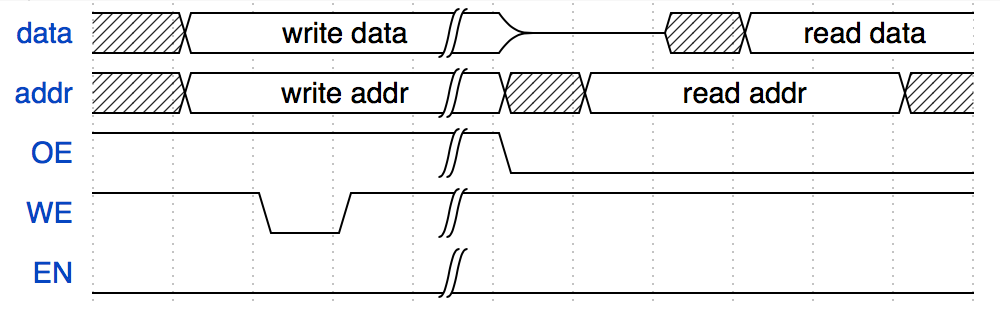
\includegraphics[width=11cm]{image/device/sram}
    \fcaption{SRAM访问时序}
\end{center}

% {signal: [
%   {name: 'data', wave: 'x2..|zx2.z', data: ['write data', 'read data']},
%   {name: 'wrn', wave: '101.|.....'},
%   {name: 'rdn', wave: '1...|.0..1'}
% ]}

\begin{center}
    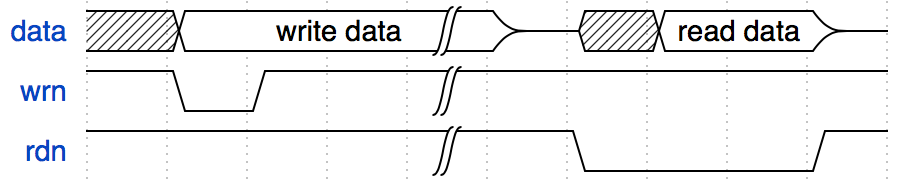
\includegraphics[width=11cm]{image/device/serial}
    \fcaption{串口访问时序}
\end{center}

% {signal: [
%   {name: 'clk', wave: '01|010'},
%   {name: 'data', wave: '2.|x..', data: ['write data']},
%   {name: 'addr', wave: '2.|2..', data: ['write addr', 'read addr']},
%   {name: 'dout', wave: 'x.|x2.', data: ['read data']},
%   {name: 'wr_en', wave: '1.|0..'},
%   {name: 'rd_en', wave: '0.|1..'}
% ]}

\begin{center}
    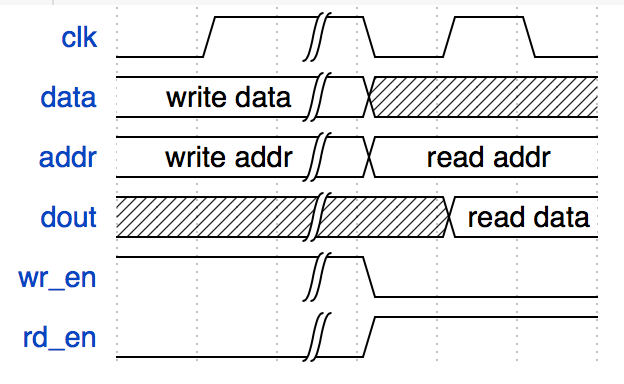
\includegraphics[width=8cm]{image/device/vga}
    \fcaption{显存访问时序(上升沿触发)}
\end{center}

% {signal: [
%   {name: 'clk', wave: '01|010'},
%   {name: 'data', wave: '2.|x..', data: ['write data']},
%   {name: 'dout', wave: 'x.|x2.', data: ['read data']},
%   {name: 'wr_en', wave: '1.|0..'},
%   {name: 'rd_en', wave: '0.|1..'}
% ]}

\begin{center}
    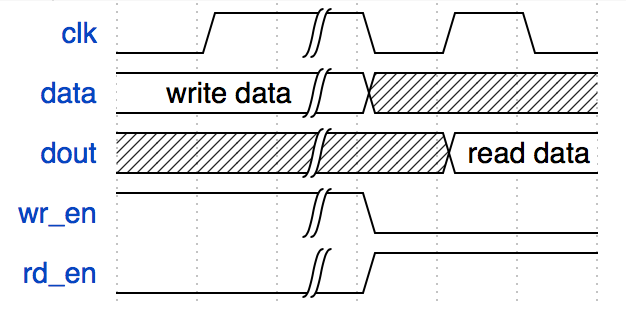
\includegraphics[width=8cm]{image/device/fifo}
    \fcaption{FIFO访问时序(上升沿触发)}
\end{center}

控制器采用两倍于CPU主频的时钟下降沿触发,分别在两个状态$S_1$与$S_2$之前跳转。对于不同访存的需求,各状态更新的控制信号如\tref{table:mem_signals}所示。初始状态下,OE, WE, rdn, wrn均为1,使能均关闭。

\begin{center}
    \tcaption{内存控制器状态转换}\label{table:mem_signals}
    \begin{longtable}{p{0.15\columnwidth}p{0.05\columnwidth}p{0.4\columnwidth}p{0.4\columnwidth}}
        \toprule
        设备 & 读/写 & $S_1$ & $S_2$ \\
        \midrule
        SRAM & 读 & OE置0,WE置1,数据线置高阻,地址线置待读取地址 & 锁存读出的数据 \\
        SRAM & 写 & OE置1,WE置1,数据线置待写入数据,地址线置待写入地址 & WE置0 \\
        串口控制 & 读 & - & 锁存输出的控制信号 \\
        串口数据 & 读 & rdn置0,wrn置1,数据线置高阻 & 锁存读出的数据,rdn置1 \\
        % 串口数据 & 写 & - & rdn置0,wrn置0,数据线置待写入数据 & wrn置0 \\
        显存地址 & 写 & 锁存地址高16位 & - \\
        显存数据 & 写 & 准备地址和数据,开启写使能,写时钟置0 & 写时钟置1 \\
        FIFO测试 & 读 & - & 锁存输出的控制信号 \\
        FIFO & 读 & 开启读使能 & 锁存读出的数据,关闭读使能 \\
        FIFO & 写 & 准备地址和数据,开启写使能,写时钟置0 & 写时钟置1 \\
        \bottomrule
    \end{longtable}
\end{center}

其中,显存与FIFO采取异步写,同步读的方式。FIFO的读时钟与控制器同频率,但是采用上升沿触发。该部件的控制信号如\tref{table:memory_ctl}所示。

\begin{center}
    \tcaption{内存控制器信号}\label{table:memory_ctl}
    \begin{longtable}{p{0.3\columnwidth}p{0.7\columnwidth}}
        \toprule
        信号 & 信号描述 \\
        clk & 控制器时钟。 \\
        rst & 异步清空信号,由外部控制开关接入。 \\
        in\_pc\_addr & 指令地址。 \\
        in\_ram\_addr & 访存地址。 \\
        in\_data & 写入数据。 \\
        in\_rd & 读使能。 \\
        in\_wr & 写使能。 \\
        out\_data & 读出数据。 \\
        out\_pc\_ins & 取出指令。 \\
        slow\_clk & CPU时钟,用于初始状态同步。 \\
        ram2\_oe & RAM2 OE控制输出。 \\
        ram2\_we & RAM2 WE控制输出。 \\
        ram2\_en & RAM2 EN控制输出。 \\
        ram2\_addr & RAM2 地址线输出。 \\
        ram2\_data & RAM2 数据总线。 \\
        ram1\_oe & RAM1 OE控制输出。 \\
        ram1\_we & RAM1 WE控制输出。 \\
        ram1\_en & RAM1 EN控制输出。 \\
        ram1\_addr & RAM1 地址线输出。 \\
        ram1\_data & RAM1 数据总线。 \\
        serial\_rdn & 串口rdn控制。 \\
        serial\_wrn & 串口wrn控制。 \\
        serial\_data\_ready & 串口data\_ready输入。 \\
        serial\_tbre & 串口tbre输入。 \\
        serial\_tsre & 串口tsre输入。 \\
        vga\_data & 显存写入数据。 \\
        vga\_addr & 显存写入地址。 \\
        vga\_data\_clk & 显存写时钟。 \\
        fifo1\_rd\_en & FIFO1读使能。 \\
        fifo1\_data & FIFO1读出数据。 \\
        fifo2\_rd\_en & FIFO2读使能。 \\
        fifo2\_wr\_clk & FIFO2写时钟。 \\
        fifo2\_data\_in & FIFO2写入数据。 \\
        fifo2\_data\_out & FIFO2读出数据。 \\
        fifo2\_is\_empty & FIFO2控制输入(是否为空)。 \\
        \midrule
        \bottomrule
    \end{longtable}
\end{center}

\section{外设和中断}

\subsection{概述}

\subsubsection{VGA像素映射的屏幕}

\begin{center}
    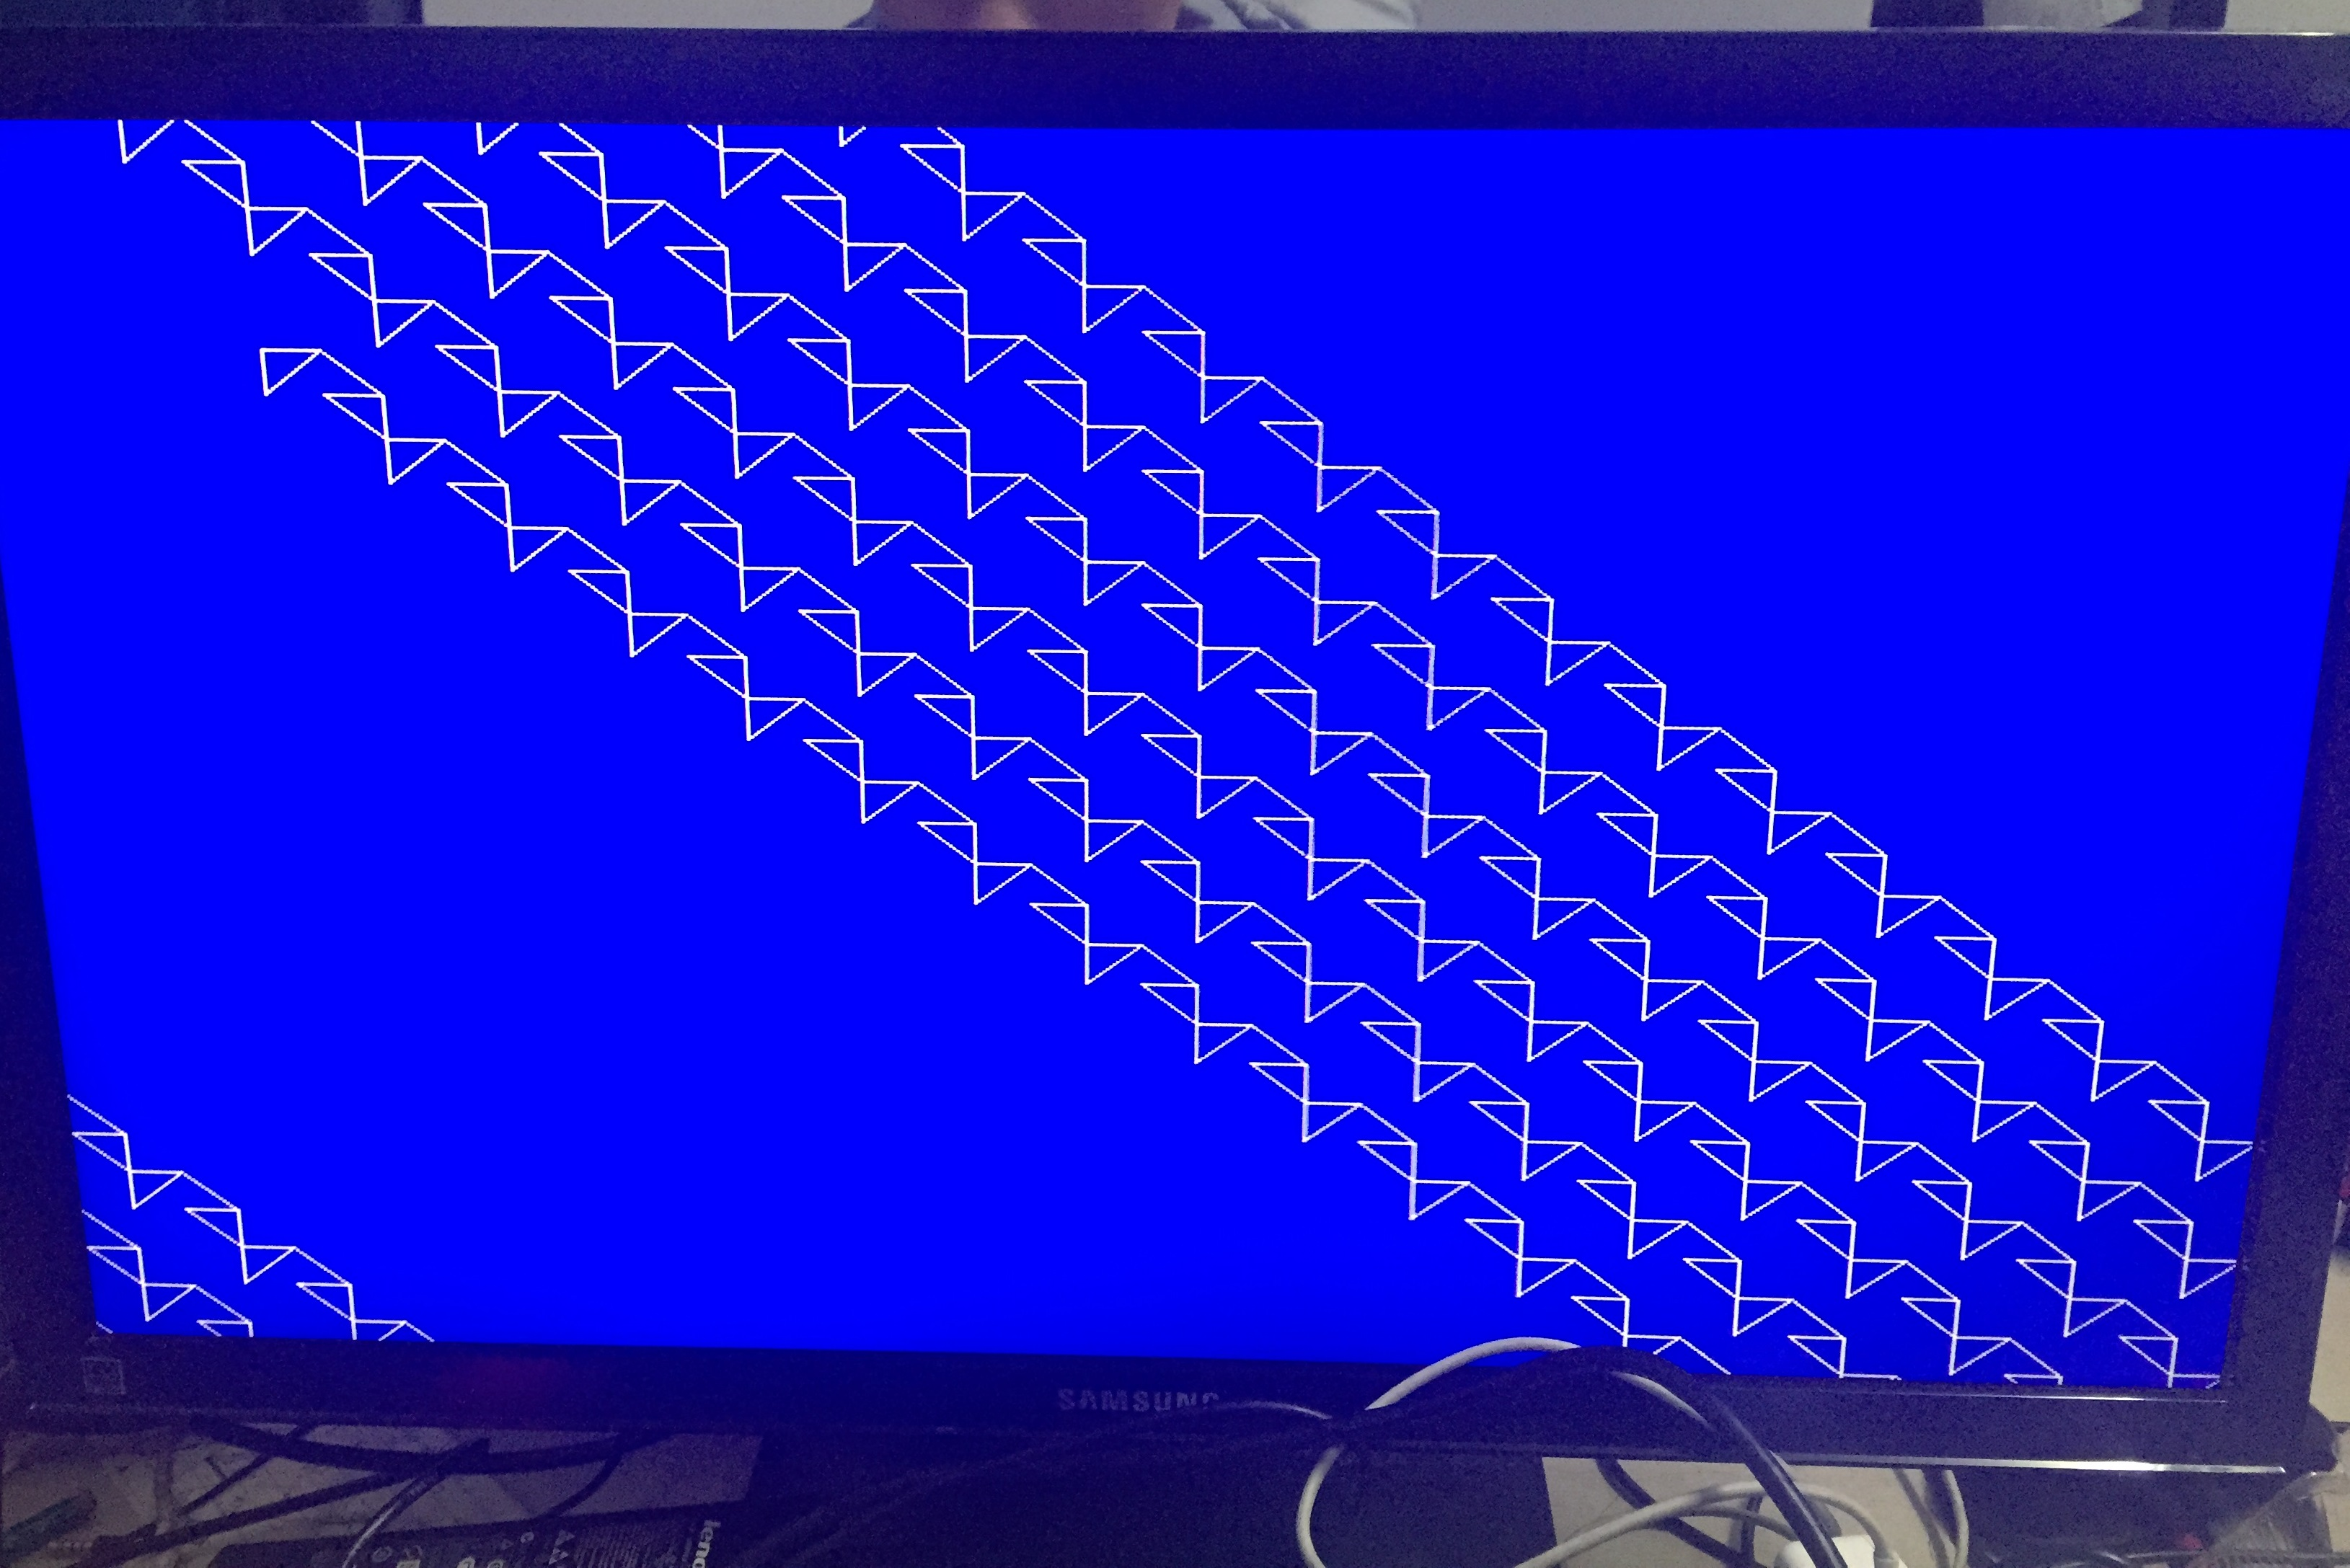
\includegraphics[height=10cm]{image/extension/tri.JPG}
    \fcaption{漂亮的三角形阵}\label{fig:ifid}
\end{center}

屏幕为像素映射。我们在片内开了一块等同于屏幕可显示像素数目大小的RAM作为我们的显存(使用ISE的IP核)。我们只需修改显存即可改变屏幕上的内容,由于片内存储空间不大,所以只能显示蓝白两色。

像素映射为我们的计算机增添了\textbf{通用性}。

\subsubsection{键盘}

\begin{center}
    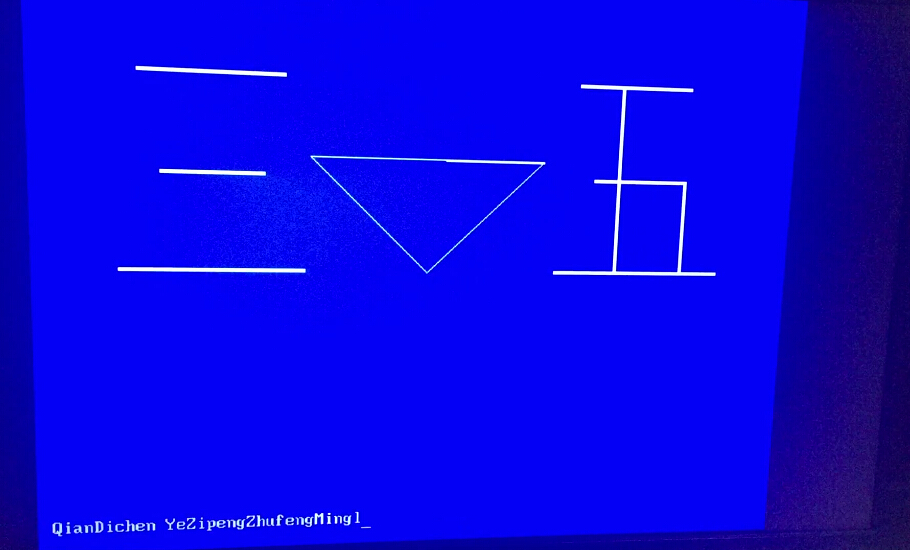
\includegraphics[height=10cm]{image/extension/35.JPG}
    \fcaption{漂亮的三角形阵}\label{fig:ifid}
\end{center}

键盘拥有2个队列:一个叫做键盘队列,给硬件中断;一个叫做软中断队列,给软件中断。键盘输入一个字符,由硬件转译成ASCII码输送给键盘队列,当队列非空并且当时不在执行中断时,发送一个硬件中断信号,执行硬件中断。由硬件中断负责把信息转译到软中断队列。

\begin{enumerate}
    \item 实现0~9,a~z,退格键,空格键,回车键。硬件将其转化为ASCII码传入键盘队列
    \item 实现shift组合键,可以发送大写的字母,以及0~9上方的特殊字符
    \item 手写实现键盘队列(长度为8),软中断队列(长度为16)
\end{enumerate}


\subsubsection{硬件中断}

硬件中断是结合键盘和中央控制器实现的。每当键盘被按下,硬件中断被触发,我们会等待MEM,和WB段执行完,清空ID和ALU段。之后记录返回PC,改变PC到中断处理程序。


\subsection{细节}

\subsubsection{VGA像素映射的屏幕}

我们将大小为$640 \times 480$的整个屏幕映射到我们的显存上,我们用1位(0或1)来表示颜色,所以我们的显存空间总共为19位。 

我们的显存使用的是ISE自带的IP核,由于片内存储空间仅稍大于屏幕的可显示像素数目,我们只映射2种颜色。我们的RAM是读写端口分开的,由CPU进行写数据,由VGA控制器读出数据显示到屏幕上。

VGA控制器,我们使用了上学期老师发给我们的VGA扫屏代码,我们在其之上进行修改。由于我们的显存只够显示两种颜色(蓝色和白色),我们用0表示蓝色,1表示白色,扫屏的时候通过判断值来给RGB的线赋值。这样我们即可从我们的显存中读出屏幕的值。

CPU通过总线来写显存。由于16位的字长不足以表示整个屏幕,我们使用2个字(BF08和BF09)来向显存控制器写一个像素点,第一个字表示地址的高16位,第二个字包括地址的地位和写入的数据的RGB(这里的RGB仅仅是留作对软件的接口,由于我们只能显示2种颜色,所以我们只用1位)。

由于对于我们的这种表示来说,写一个模式(一个字母或者一个图形)对软件的要求极高,我们的工作有一部分也体现在软件上。这体现了我们的硬件的通用性,也考验我们硬件的鲁棒性。


\subsubsection{键盘,键盘队列以及软中断队列}

键盘的控制器是由上学期老师发的键盘代码修改而成的。

我们的键盘控制器能把通码转成ASCII码,滤去键盘不停发送的通码,直到接收到断码为止,也就是说我们的键盘不会导致失误。除此以外,我们支持组合键(shift + 按键可以产生大写的ASCII码),空格键,回车键,退格键······

键盘队列和软中断队列都是由我们自己实现。

这个队列是我们定义的一个模块,有2个端口,一个端口用于入队(写队列),一个端口用于出队(读队列)。每个端口都有各自的时钟(异步读写)和各自的使能端(如果不使能则队列保持不变)。队列内使用触发器存储数据,使用两个计数器来计数,分别表示队首和队尾。如果队首等于队尾则队列为空,否则队列非空,此时中断队列会发出中断信号,中央控制器会响应中断。

入队过程由上升沿触发,出队过程也是上升沿触发。是否入队/出队由入队/出队使能决定。键盘队列的容量是8个字,软中断队列的容量是16个字。

\subsubsection{硬中断}
我们每次按下键盘,键盘会将通码转换成ASCII码入队。这时队列的非空信号会触发一个硬件中断(由中央控制器实现)。

此时中央控制器会响应硬件中断,这是一个复杂的过程,整个流程分为如下几步:

\begin{enumerate}
    \item 锁住PC的写使能
    \item 存下EPC
    \item 清空流水线
    \item 跳转到中断处理程序
    \item 执行中断
    \item 中断返回
\end{enumerate}

我们详细说明如何清空流水线以及如何中断返回。

确定EPC:我们会先检查ID/ALU阶段寄存器的PC值是否为全0,如果不全0,我们将选择它。否则选择IF/ID段的PC值。为什么这样取呢?因为ID/ALU段可能是气泡,如果全0肯定是气泡,我们不能使用它。而我们整个流水线中不可能有连续2个气泡存在,所以选择IF/ID是安全的。

清空流水线:由于我们有分支预测,有插气泡的可能,我们认为流水线全部清空是不合适的。因为这时如果有分支预测错误,将不能复原。我们认为让流水线流完也是不合适的,此时PC的使能被锁住,如果有跳转将不能正常跳转。我们选择了一个折衷的方法,也是MIPS提倡的方法,把MEM和WB段的指令执行完,而ID和ALU段的指令清空。这样在我们的架构下不会产生冲突,中断得以正常进行。

中断返回:我们新增了一条ERET指令,代码是  FFFF  ,这条指令是中断执行程序的特权指令,只有在中断正在执行的时候才有效。这条指令会相当于一条B  EPC  ,表明中断执行结束,需要继续执行指令。

\subsubsection{软中断}
由软件实现,其过程需要等待硬中断的触发以及处理,通过硬中断把键盘队列中的数据转移到软中断队列中,软中断得以结束。

\section{软件方面}

\subsection{针对我们像素映射实现的接口}

\begin{enumerate}
    \item 给定坐标画一个点
    \item 给定起始点,长度,类型(总共8个类型,每45度角为一类)画一条细线段
    \item 给定起始点,长度,类型(同上),粗细,画一条粗线段
    \item 给定直角顶点,大小,类型(总共8个类型,每45度角为一类)画一个等腰直角三角形
    \item 从数据RAM中读取一个形状(用于实现字符集,比如汉字或是ASCII码)
\end{enumerate}




\subsection{针对键盘实现的硬件中断和软件中断的中断程序}

\subsubsection{硬件中断}

\begin{enumerate}
    \item 从键盘输入队列中取出一个ASCII码输出到串口
    \item 从键盘输入队列中取出一个ASCII码输入到软中断队列
    \item 从键盘输入队列中取出一个ASCII码,通过调用字符显示的函数显示到屏幕
    \item 实现退格键
\end{enumerate}

\subsubsection{软件中断}

(类似于scanf()  ,  支持char 和 int)
\begin{enumerate}
    \item 从软件中断队列中读取一个ASCII码
    \item 从软件中断队列中读取一串数字,直到空格,并解析成一个INT
    \item (暂未完成)完成一个画图程序,读入画图指令,解析成参数,传给画图函数实现画图的功能,由于时间紧张,汇编代码(1000+行)已经完成,然后没有调试完全,还不能工作。
\end{enumerate}

\subsection{定制的term}

\subsubsection{概述}
由于老师提供的term只支持基础指令,而我们需要调试也需要使用扩展的指令。

\subsubsection{具体内容及实现}
我们自己的Term具备老师的Term的全部功能,除此以外,我们为它增添了新的特性,包括:
\begin{enumerate}
    \item 可以识别拓展的5条指令,包括NOT,BTNEZ,SLT,JALR,JRRA
    \item 可以向RAM中写入拓展的5条指令,包括NOT,BTNEZ,SLT,JALR,JRRA
    \item 中断的支持,对ERET的写入
\end{enumerate}

实现这个term的过程并不难,因为莱斯提供了term的源码,我们只需要在其A指令和U指令的模块中增加我们的指令即可。



\section{测试}

\subsection{性能测试}

我们在监控程序中对所提供的5个流水线性能测试程序进行测试,得到的结果如\tref{table:per_test}所示。CPU主频为20MHz。

\begin{center}
    \tcaption{流水线性能测试结果}\label{table:per_test}
    \begin{longtable}{cccc}
        \toprule
        测试程序 & 运行时间 (s) & 指令条数 (亿) & CPI \\
        \midrule
        1 & 6.257 & 1.25 & 1.001 \\
        2 & 10.005 & 2.00 & 1.000 \\
        3 & 4.992 & 1.00 & 0.998 \\
        4 & 4.993 & 1.00 & 0.999 \\
        5 & 4.994 & 0.75 & 1.332 \\
        \bottomrule
    \end{longtable}
\end{center}

可见,除了读写指令内存需要插气泡,导致CPI增加以外,其他程序运行的CPI都接近于1,说明数据旁路对于冲突处理得很好,只有在少数情况下才需要暂停流水线。

\subsection{扩展指令测试}

我们编写了两段程序用于测试扩展指令的正确性。

\subsubsection{扩展指令测试程序1}

程序源码为

\lstset{basicstyle=\small\ttfamily, numbers=left}
\begin{lstlisting}
    LI R0 40
    SLL R0 R0 0
    ADDIU R0 0A
    LI R1 0
    LI R2 0
    LI R3 0
    LI R4 0
    JALR R0
    JR R7
    NOP
    NOT R1 R1
    NOT R2 R2
    NOT R3 R3
    NOT R4 R4
    JRRA
    NOP
\end{lstlisting}

这段程序的功能是:置R0至R4为0,然后通过JALR指令进行过程调用,跳转到0x400A,即这里的第10行,从而完成把R1至R4分别取反赋给它们自己,即变为0xFFFF。运行前后寄存器值如\fref{fig:testp1}所示,说明结果正确。

\begin{center}
    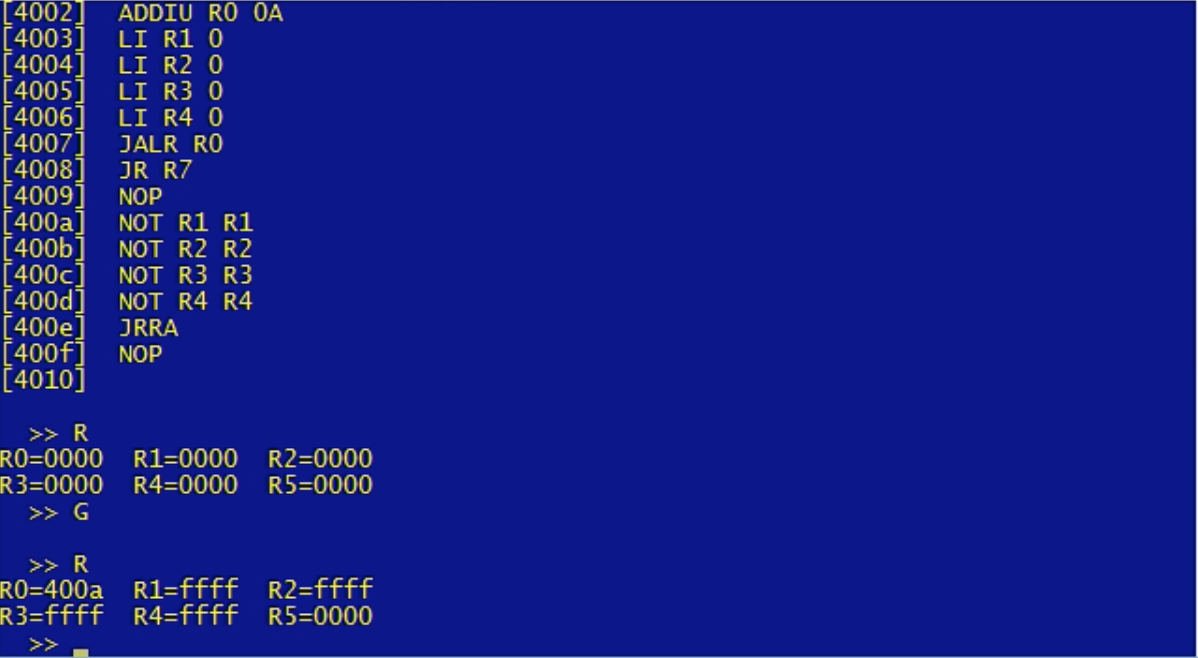
\includegraphics[width=13cm]{image/testing/p1}
    \fcaption{测试程序1运行结果}\label{fig:testp1}
\end{center}

这段程序验证了\texttt{NOT}, \texttt{JALR}, \texttt{JRRA}的正确性。

\subsubsection{扩展指令测试程序2}

程序源码为

\begin{lstlisting}
    LI R0 1
    LI R1 2
    SLT R0 R1
    BTNEZ 5
    NOP
    LI R3 80
    JR R7
    NOP
    LI R5 0
    NOT R5 R5
    SLT R1 R0
    BTNEZ FA
    NOP
    JR R7
    NOP
\end{lstlisting}

这段程序的功能是:置R0为1,置R1为2。第3行处由于R0<R1,置T为1。由于T不等于0,第4行的跳转会被执行。即从第9行开始执行,R5先被置0,然后取反,结果为0xFFFF。之后由于R1>R0,故第12行的跳转不会执行,直接退出用户程序,返回监控程序。假设第12行跳转执行,那么在第6行R3会被赋值为0x80。运行前后寄存器值如\fref{fig:testp2}所示,R3的值未改变,而R5变成0xFFFF,说明结果正确。

\begin{center}
    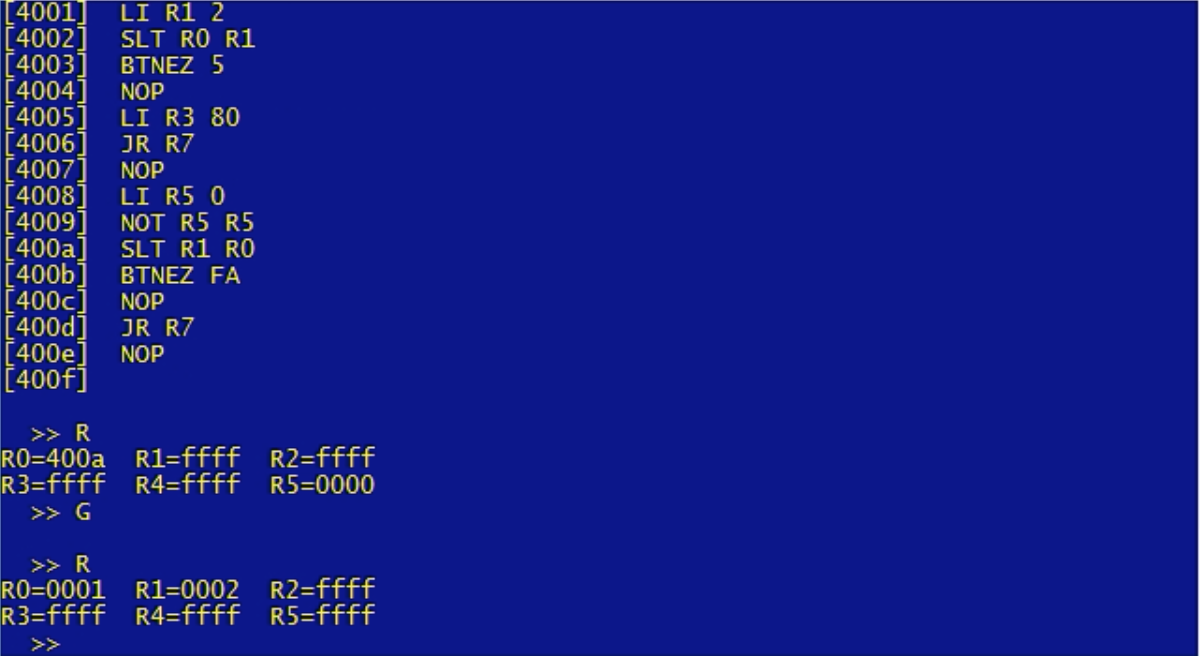
\includegraphics[width=13cm]{image/testing/p2}
    \fcaption{测试程序2运行结果}\label{fig:testp2}
\end{center}

这段程序验证了\texttt{SLT}, \texttt{BTNEZ}的正确性。

\subsection{外设与中断测试}

这部分我们采用了一个绘图程序用来展示VGA的像素映射功能与键盘输入功能。由于是硬件中断,我们可以发现在键盘输入后屏幕上会立即响应,同时已经绘制好的图形也不受影响。如\fref{fig:vga_keyboard}所示。

\begin{center}
    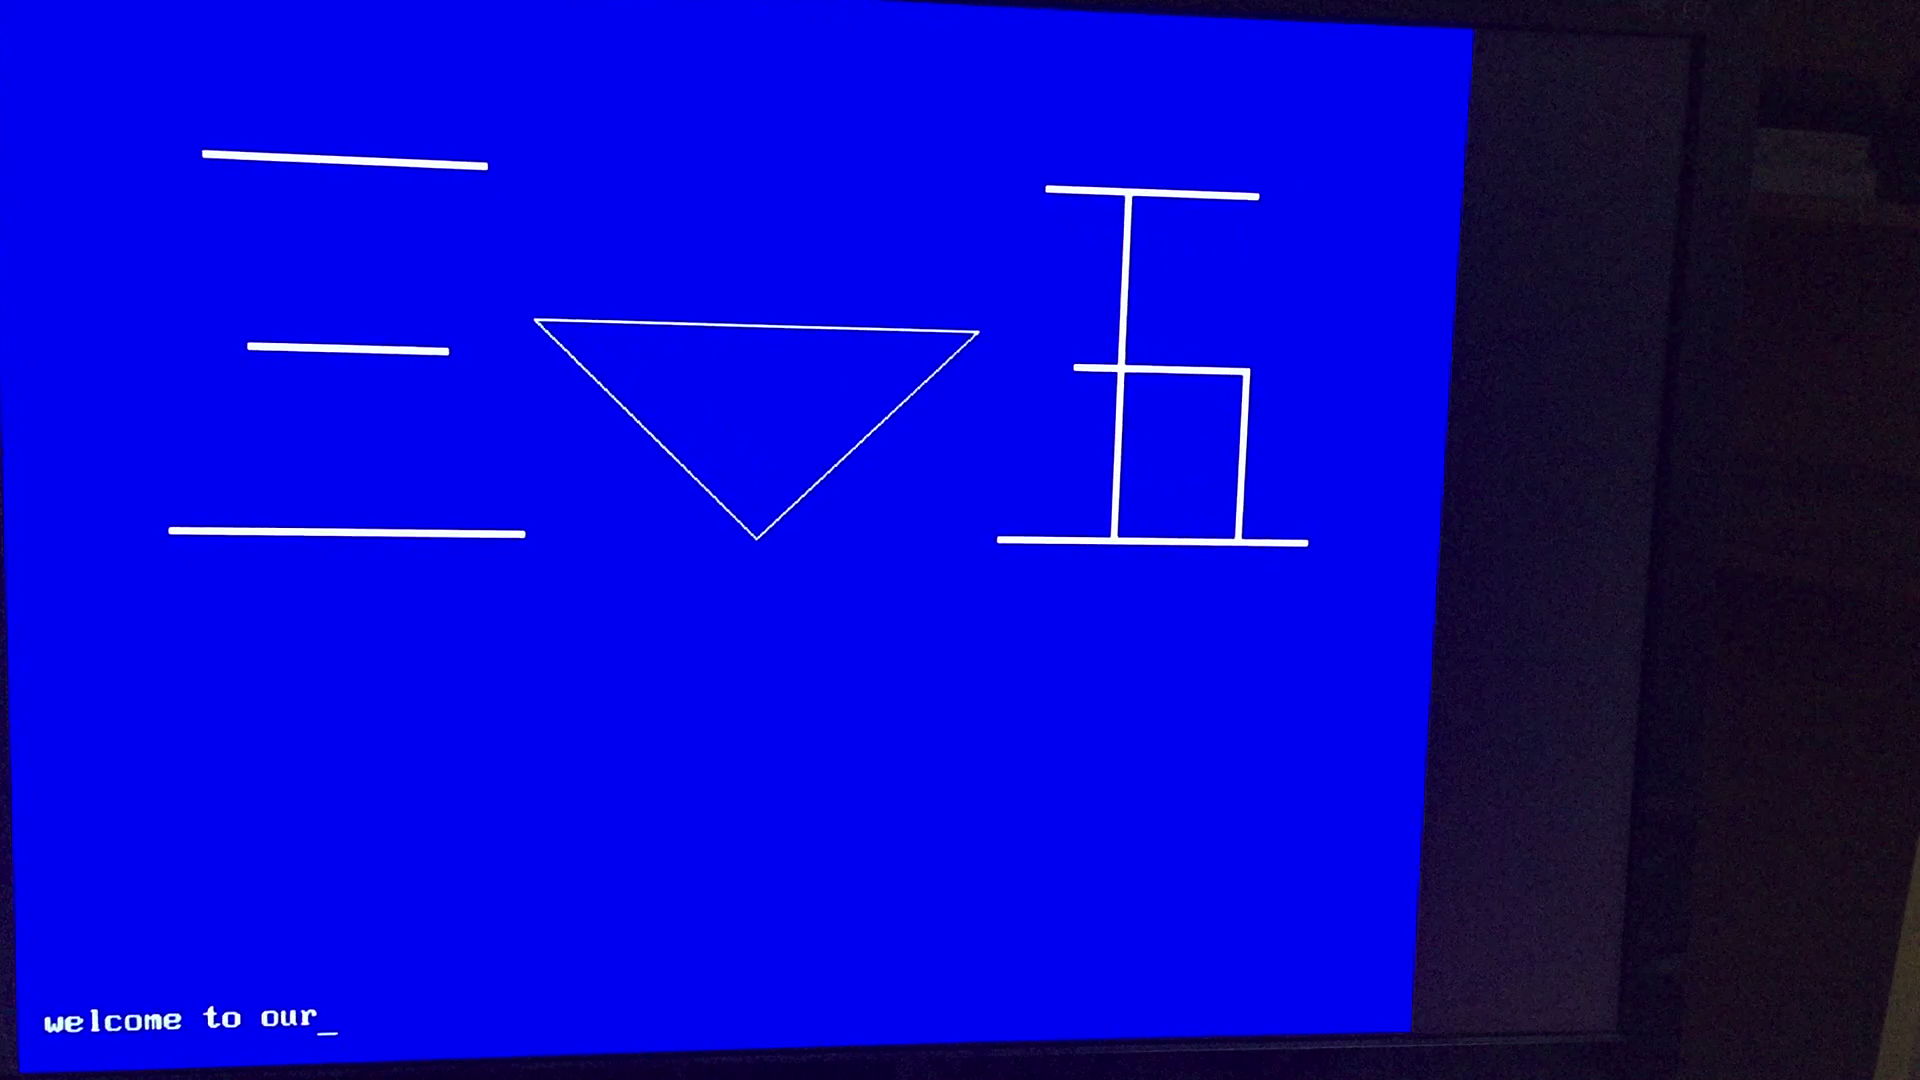
\includegraphics[width=13cm]{image/testing/vga_keyboard}
    \fcaption{外设演示}\label{fig:vga_keyboard}
\end{center}

键盘不仅可以输入,还可以按空格键清除输入的内容。

\begin{center}
    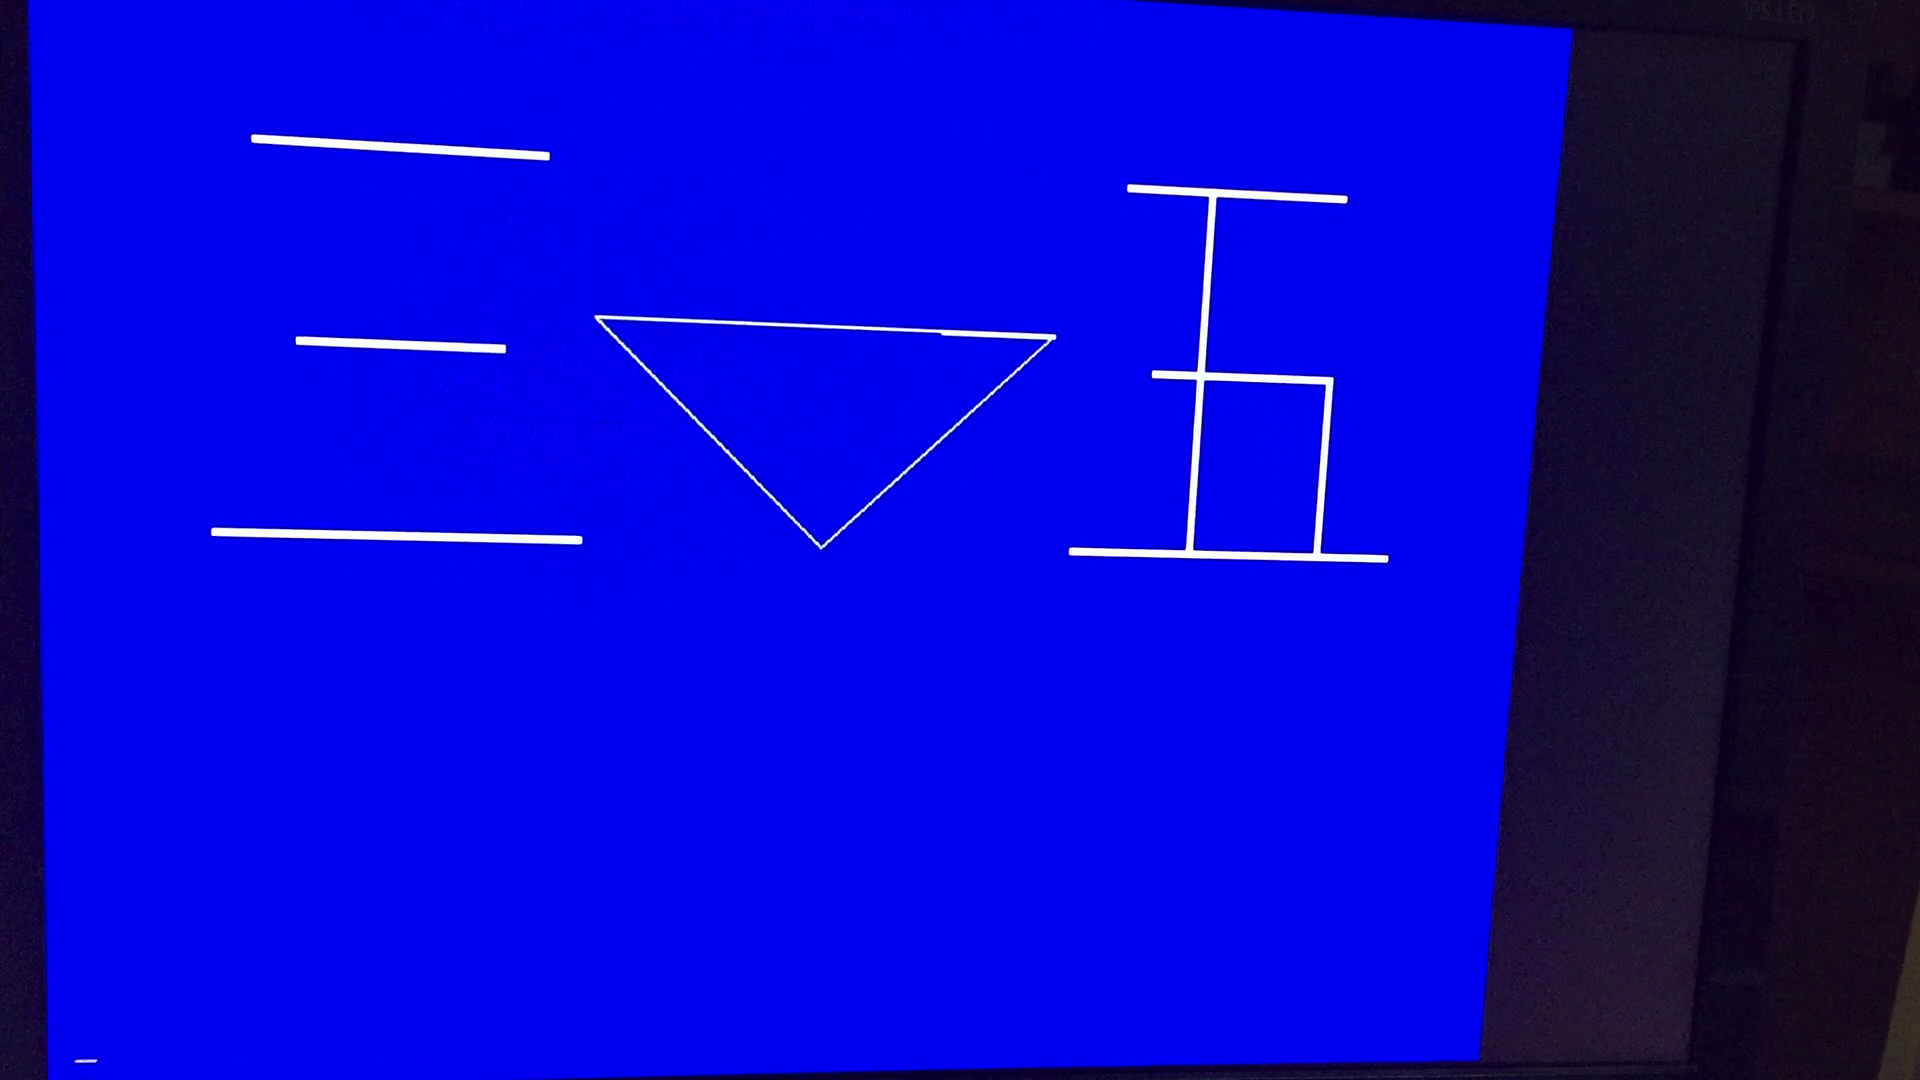
\includegraphics[width=13cm]{image/testing/clear}
    \fcaption{按空格键清屏}
\end{center}

此外,键盘还支持大小写输入。即,键盘不仅能捕获到单个键,还能捕获到组合键,如输入大写的A则在按下SHIFT键同时按下A。

\begin{center}
    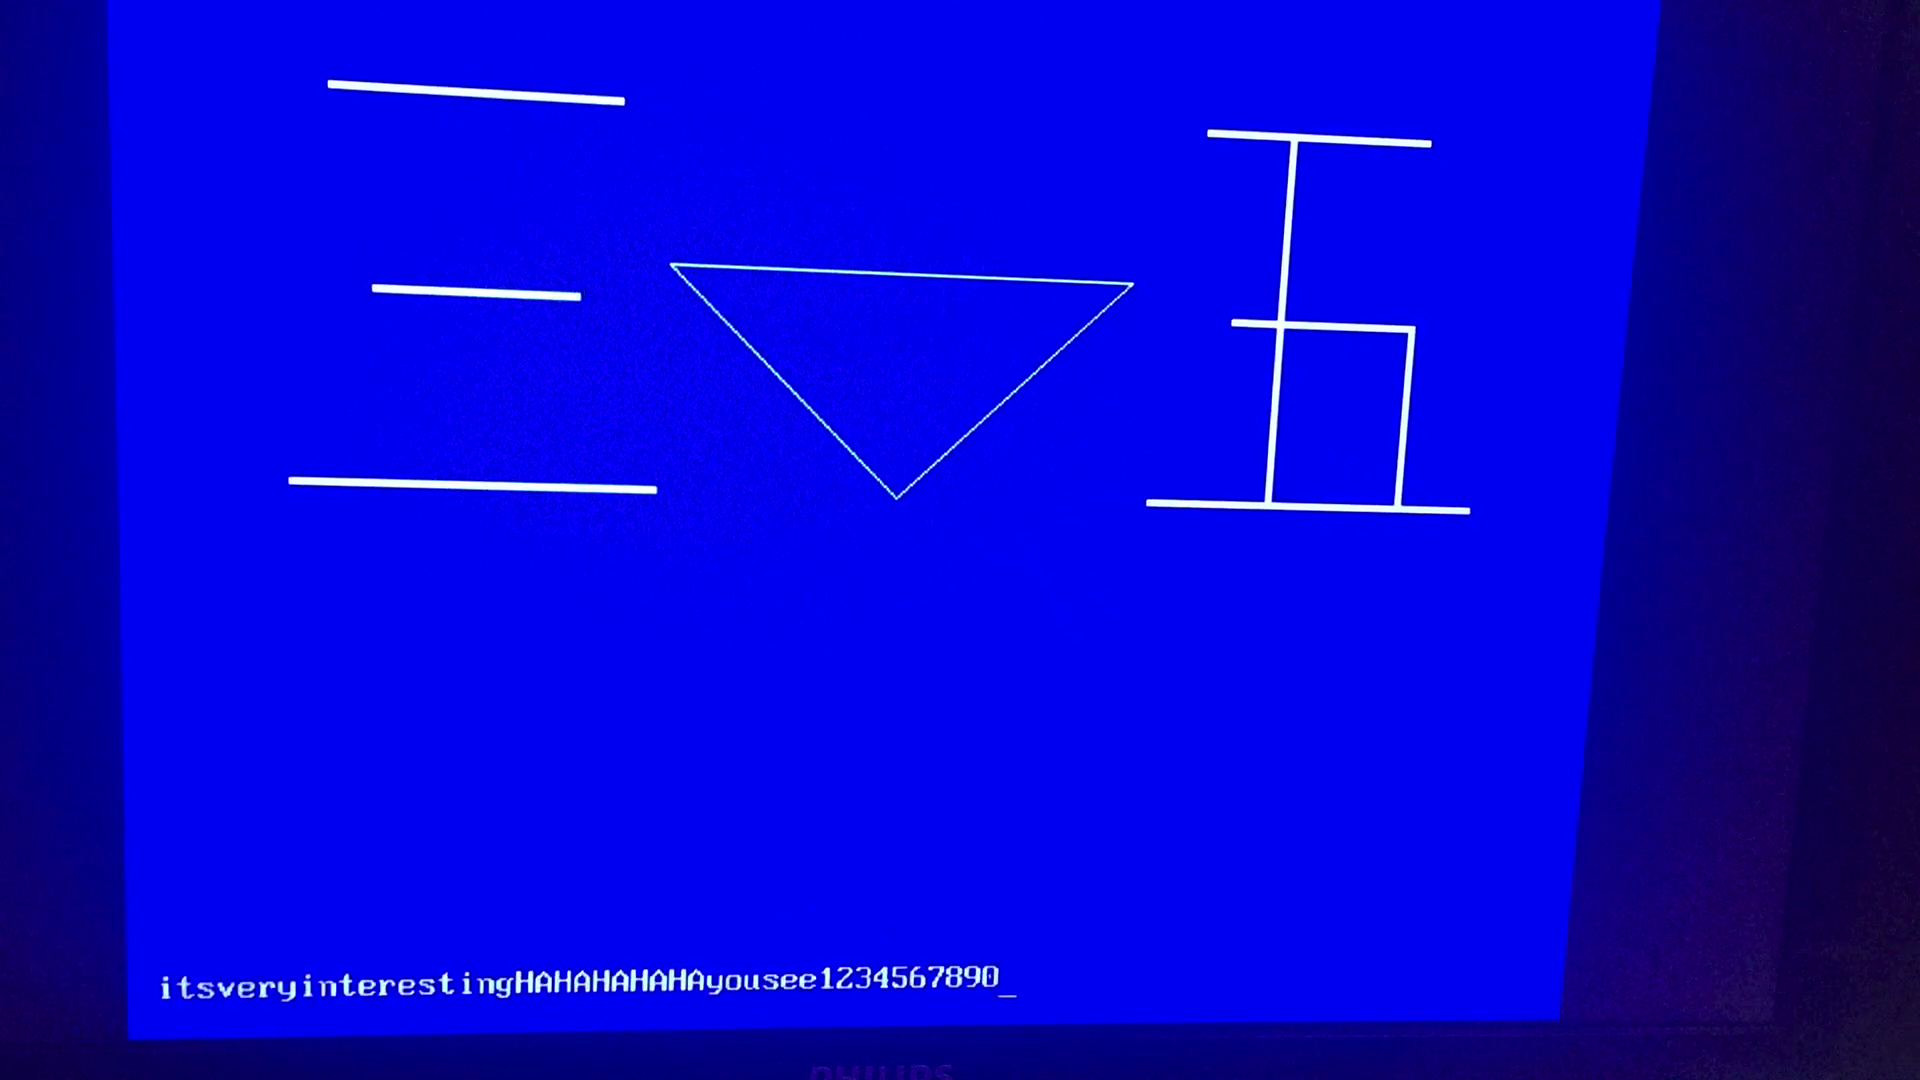
\includegraphics[width=13cm]{image/testing/case}
    \fcaption{大小写字符均可输入}
\end{center}

当输入错误时还可以按退格键删除一个字符。

\begin{center}
    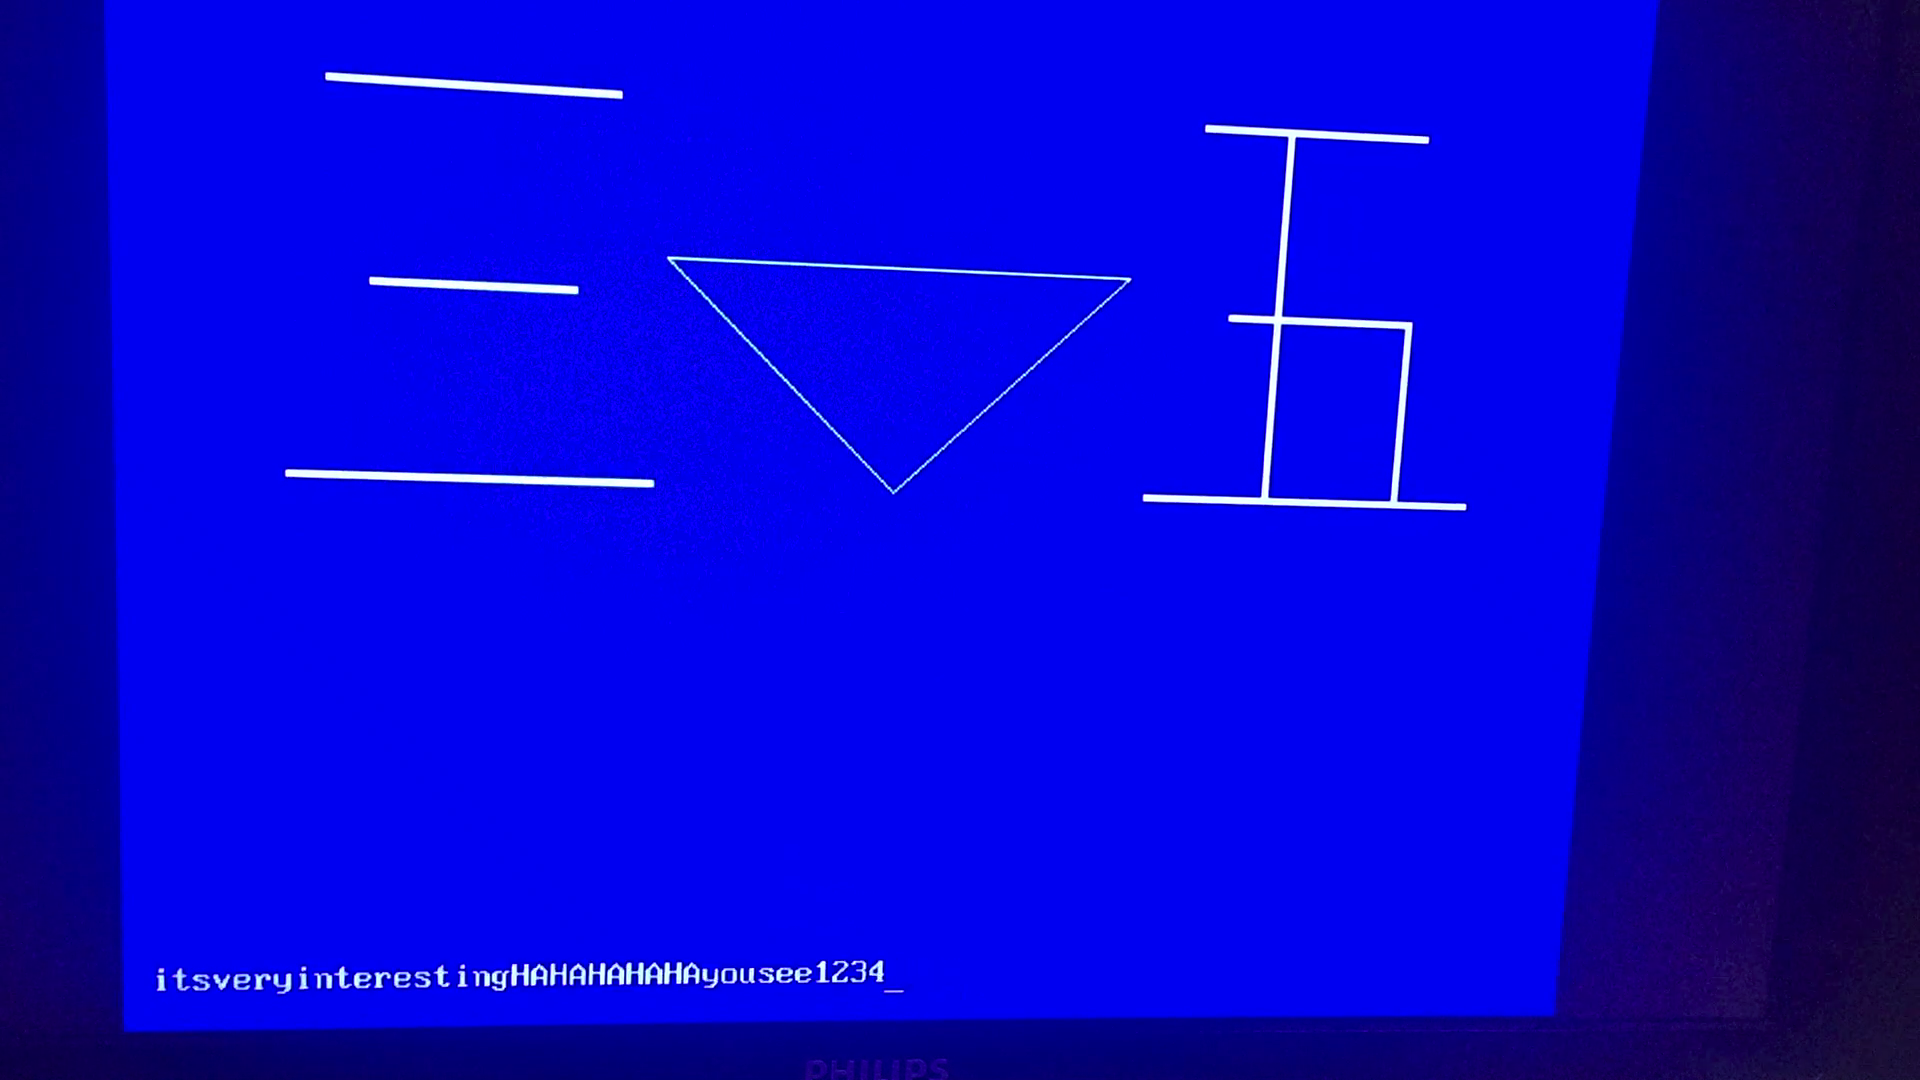
\includegraphics[width=13cm]{image/testing/backspace}
    \fcaption{退格}
\end{center}

至此,我们实现的所有30条指令以及自己扩展的\texttt{ERET}指令均通过了测试。

\section{越过的千难万险}

\subsection{奇偶校验}

在单独调试串口的时候,助教早已告诉了我们,要开奇校验。由于我们一直没遇到问题,所以一直都没开奇校验。突然某一天,我们的串口突然不能正常工作了,连续两条串口发来的消息总会有一条出错。我们百思不得其解,我们仔细研究了其出错的情形,寻找出错数据的共同点,最后终于发现了原因。

\subsection{奇妙的A指令}

刚开始的时候,我们的A指令总是只能写一条指令,每次写多条的时候,后面的指令都写不进去。

于是我们便开始了单步调试,单步的Term根本无法运行,我们只好使用串口模拟Term的行为,Term给串口发什么,我们就给串口发什么。我们按照源码自己解读收到的串口信息。经历了千辛万苦之后,终于尝到了甘泉。我们发现有一个地方的控制出了差错,原来是在修改指令RAM的时候,有一种情况没有插气泡。发现了这个错误,我们欣喜若狂,立即修改了这个BUG,于是我们的Term算是可以运行了。

\subsection{虚妄的加速}

我们的CPU不能运行在25M主频下。这一点很令我们头疼。

我们研究了ISE给我们的时间分析和时间报告,找到了关键路径。

我们开始报告24M,我们想办法增加到了29M,又提高到了36M,最后报告达到了46M。我们加了各种时间约束,各种约束都通过了。然而最后我们的CPU依然承受不住25M的洗礼。我认为可能是我们的板子延迟略高于标准值,或者是其它的什么原因导致的。

我们最后只能跑在21M的主频下。老师说21M和25M差不太多,我们对于旁路和分支预测的处理很好,这已经足够了。



\end{document}
% -----------------end------------------%
